\documentclass[american]{i3thesis} % Sets American English as the document language

% CRITICAL: Force biblatex options before the class loads them
\PassOptionsToPackage{style=numeric,sorting=none,backend=biber,language=american}{biblatex}

% Fix for the date issue - force the use of thethesisend instead of \today
\makeatletter
\renewcommand{\thedate}{\thethesisend}
\makeatother

% CRITICAL: Add this to select American English as the main language
\selectlanguage{american}

% Add unicode character support
\usepackage{textcomp}
\providecommand{\declarationname}{Declaration}

% Load packages without conflicting options
\usepackage{multirow}
\usepackage{floatflt}

% Add float control packages
\usepackage{float}
\usepackage{placeins}

% Fix for unicode characters
\usepackage{newunicodechar}
\newunicodechar{≠}{\ensuremath{\neq}}

% Set variables for the document
\author{Ashwin Varkey}
\title{A SystemC-Based Implementation of an IEEE 754 Pipelined Floating-Point Unit with Zynq FPGA Verification}

% Required for non-German thesis
\germantitle{A SystemC-Based Implementation of an IEEE 754 Pipelined Floating-Point Unit with Zynq FPGA Verification}

% Remove "in" from thesis type by using "of" instead of "in"
\thesistype{Master's Thesis in Computational Engineering}
\thesiscite{Master's Thesis, University of Erlangen, Dept. of Computer Science, June 2025}
\birthday{30. January 1998}
\birthplace{India}
\thesisstart{10. December 2024}
\thesisend{10. June 2025}
\advisors{Prof. Dr.-Ing. Dietmar Fey}

% Patch the location text to remove "in" before birthplace
\makeatletter
% Patch the master thesis title page to remove "in" before birthplace
\let\original@maketitle\maketitle
\renewcommand{\maketitle}{%
  % Save the original definition of "in"
  \let\original@in\in
  % Redefine "in" to be empty only in the context of "geb. am X in Y"
  \renewcommand{\in}{}%
  % Call the original maketitle
  \original@maketitle
  % Restore the original definition of "in"
  \let\in\original@in
}
\makeatother

% Redefine chapter and section related names to force English
\AtBeginDocument{%
  \renewcommand{\chaptername}{Chapter}
  \renewcommand{\contentsname}{Table of Contents}
  \renewcommand{\listfigurename}{List of Figures}
  \renewcommand{\listtablename}{List of Tables}
  % Fix for "Abbildung" and "Tabelle"
  \renewcommand{\figurename}{Figure}
  \renewcommand{\tablename}{Table}
}

% Load hyperref at the end
\usepackage{hyperref}
\hypersetup{pageanchor=true}

\addbibresource{thesis.bib}
\graphicspath{{figures/},{images/},{pictures/}}

\begin{document}
\pagenumbering{roman}

% Let the i3thesis class generate the cover page with logo
\maketitle

% We don't need to create a second English title page since we're already using an English thesis
% The default title page will be in English due to the 'american' option in the document class

% Reset the page counter for roman numbering
\setcounter{page}{1}

% Since we're using an English thesis, we don't need the Declaration page again
% It's already generated by the class with the English text
% If you want to customize it further, uncomment and modify this section:
%
% \begin{center}
% \textbf{\Large Declaration}
% \end{center}
% \vspace{1cm}
% I declare that the work is entirely my own and was produced with no assistance from third parties. I certify that the work has not been submitted in the same or any similar form for assessment to any other examining body and all references, direct and indirect, are indicated as such and have been cited accordingly.
% \vspace{2cm}
% \begin{flushright}
% \rule{6cm}{0.5pt}\\
% (Ashwin Varkey)\\
% Erlangen, 10. June 2025
% \end{flushright}

\acresetall
\cleardoublepage
\tableofcontents
\cleardoublepage
\pagenumbering{arabic}

\chapter*{Abstract}
\addcontentsline{toc}{chapter}{Abstract}

Floating-point arithmetic units are a fundamental component in modern processor architectures, and RISC-V open standard approach to floating point extensions provides a simplified model for implementing IEEE 754 compliant operations in a pipeline structure. The IEEE-754 standard ensures consistency and computational accuracy defines the specific formats and operations that hardware implementations must follow for proper floating-point computation.

This research presents a floating-point processor that implements standard arithmetic units-adder, multiplier, subtractor and divider within a five-stage pipeline structure. The fetch and decode components for the floating-point unit were developed using the rv32f extensions of RISC-V Instruction Set Architecture (ISA). The initial stage includes SystemC modeling followed by Register Level Transfer (RTL) design which comes from synthesis and simulation before the development of a prototype that will be implemented in Field Programmable Gate Array (FPGA) board.

To ensure the design worked correctly, a custom testbench was created with a wide range of inputs and edge cases covering all the arithmetic limits. The floating-point units received improvements through instruction level simulation results. Detailed waveform analysis revealed instruction control behaviors and facilitated solving the execution anomalies. The RISC-V ISA simulator Spike served as a cross-verification tool to execute test benches that originated from the RISC-V GCC toolchain and was compared with our floating-point unit results. 

This methodology allows quick development cycles without affecting performance providing a template that joins high level synthesis (HLS)  with simulator based verification before hardware deployment.
\chapter{Introduction}
\label{chap:introduction}

System on Chip design complexity has surged requiring the need for advanced methodologies like high level synthesis (HLS) which facilitate faster design through high-level programming languages such as C/C++ and SystemC~\cite{ref1}. While HLS has proven effective for application-specific accelerators, its application to general-purpose processors has been limited due to challenges in handling control-dominated logic. Floating point units are important for processor architecture development enabling precise representation and manipulation of real numbers which advance computing performance~\cite{ref2}.

The IEEE 754 standard is used to establish consistency and computational accuracy with specific formats and operations that hardware implementations must adhere to for reliable floating-point computations~\cite{ref3}. The design and implementation of custom-floating point units present several challenges, taking inspiration from RISC-V pipeline ensuring compliance with IEEE 754, managing pipeline hazards and optimizing for the FPGA board. Addressing these obstacles requires a comprehensive approach that spans high-level architectural modelling, detailed RTL implementation and thorough verification methodology.

As computational demands continue to increase particularly in embedded computing environments, the efficient hardware implementation of floating-point operations is important. While regular computer processors have built-in components for handling decimal calculations, they are designed to be all-purpose rather than specialized for specific tasks~\cite{ref4}. If you are working on applications with strict speed, power or resource requirements, custom floating-point designs on reconfigurable hardware like FPGAs can offer major benefits by optimizing the architecture and fine tuning the processing pipeline.

In programming terms, FPGA plays the role of personal computer while High Level Synthesis Tool acts like the C compiler. It gives access to the FPGA through high level language. Zynq XC7Z020 from Xilinx is a SOC containing several components: processors, memories, USB and Ethernet interfaces whose programmable part contains 6650 Configurable Logic Blocks (CLB).~\cite{ref3}

The increasing use of heterogenous computing boards starts a new revolution for customised floating point processor with the gap between high level algorithm and hardware implementation being addressed sufficiently. \cite{ref6}

\section{Motivation and Problem Statement}
\label{sec:motivation}

Despite advances in processor architecture and digital design methodologies several challenges persist in efficient implementation of floating-point units~\cite{ref7}:

\begin{itemize}
\item Conventional floating-point implementation often struggles to achieve high accuracy, low latency and efficient resource utilization.
\item The detailed implementation of IEEE 754 compliant operations, especially division and special case handling, introduces a complexity that must be carefully managed to ensure correctness.
\item Transitioning from high-level programming languages to hardware description languages (HDLs) requires adapting to fundamentally different design paradigms and hardware-specific constructs.
\item Comprehensive verification of floating-point operation requires sufficient test coverage across normal and special cases requiring proper verification methodologies.
\item Implementing floating point units on specific FPGA platform introduces additional considerations like available pinouts, clock frequency limits and integration with existing board design.
\end{itemize}

\section{Research Objectives}
\label{sec:objectives}

This research aims to achieve the following objectives:

\begin{itemize}
\item Design and implement a five-stage pipeline for IEEE-754 standard floating point operations including addition,subtraction,multiplication and division
\item Develop a comprehensive SystemC model that allows us to explore different architectural options, analyze accuracy and functionality before moving to detailed RTL implementation phase
\item Develop a practical verification that confirms computational accuracy across normal operations, special cases and boundary conditions for all floating-point units
\item Implement floating point unit on Xilinx Zynq using Vivado with careful resource utilization and integration with existing system components
\end{itemize}

\section{Development Environment and Tools}
\label{sec:dev_environment}

The floating-point unit implementation leveraged a comprehensive development environment spanning:

\subsection{High-Level Modeling Environment}
\begin{itemize}
\item \textbf{SystemC Library:} Version 2.3.3, providing transaction-level modeling constructs and simulation kernel
\item \textbf{C++ Compiler:} GCC 9.3.0 with C++14 standard support for compilation and linking
\item \textbf{Build System:} CMake 3.16, managing cross-platform build configuration and dependency resolution
\end{itemize}

\subsection{RTL Design and Synthesis Tools}
\begin{itemize}
\item \textbf{Xilinx Vivado 2019.2:} Primary tool for RTL synthesis, implementation, and FPGA targeting
\item \textbf{Intel Compiler for SystemC (ICSC):} High-level synthesis tool that translates synthesizable SystemC code into SystemVerilog.
\end{itemize}

\subsection{Verification and Analysis Tools}
\begin{itemize}
\item \textbf{GTKWave 3.3.104:} Waveform visualization and signal analysis for debugging
\item \textbf{RISC-V GNU Toolchain:} Cross-compiler and assembler for generating test programs
\item \textbf{Spike RISC-V ISA Simulator:} Reference implementation for golden model comparison
\end{itemize}

\subsection{Development Infrastructure}
\begin{itemize}
\item \textbf{Documentation:} LaTeX with TeXstudio for technical documentation
\item \textbf{Hardware Platform:} Xilinx Zynq XC7Z020 evaluation board for implementation validation
\end{itemize}

\section{Literature Review}
\label{sec:literature_review}

The literature review sets the theoretical foundation for this thesis topic and mentions concepts for floating point arithmetic, pipelined architecture, and FPGA implementation. The search uses peer reviewed journals, conference papers, technical standards (IEEE 754), and reference texts published in the past two decades. Academic databases like IEEE Xplore, ACM Digital Library, Science Direct, and Google Scholar, employing keywords related to floating-point hardware, pipelined processors, SystemC modeling, and FPGA implementation. 
Floating point representation allows computers to work with real numbers, addressing limitations of fixed arithmetic where a fractional is used for storing a certain fixed number of digits. The IEEE 754 standard was established in 1985 and revised twice in 2008 and 2019 to account for changes and improvements suggested by scholars.Recent work by Jaiswal and So examines implementation changes specific to floating point addition, proposes a method that minimizes the critical path through optimized normalization and rounding~\cite{ref8}. Similarly, Dinechin and Pasca address multiplication optimization algorithm through specialized significand multipliers and exception handling logic~\cite{ref9}. 
SystemC is a very important programming language for hardware modelling and simulation. Grotker et al. explains the SystemC modeling approach, describing its ability to represent hardware to the lowest level of digital circuits~\cite{ref11}. For floating point units, Reshadi et al.'s work describes both functional and timing behavior~\cite{ref12}. High level synthesis (HLS) has picked up a lot of significance in hardware design. Goossens studies the path from algorithmic to hardware implementation, helping developers to feature processor parts at high abstraction level~\cite{ref13}. HLS struggles with optimising peak performance and resource efficiency despite making designing easier. The solution Goossens suggests is manual debugging, which is a hybrid approach with HLS for fast prototyping and targets RTL level fine tuning~\cite{ref13}.
The Xilinx Zynq platform gives significant advantages and challenges for floating point implementations with both programming and embedded logic being involved. Crocket et al. gives a proper description of Zynq architecture, describing communication mechanisms between processing system (PS) and programming logic (PL) parts~\cite{ref14}. Comprehensive verification of the floating point hardware will require a testbench of basic, special and boundary operations/testcases. Verma et al. give a simple way to floating point operations that cover underflow and overflow with an emphasis on randomised testing~\cite{ref15}.
The literature review exposes several gaps and opportunities to look into floating point processor design and implementation. While a lot of research explains individual floating point designs in high level programming languages like Python and Verilog/VHDL, integrated methodologies that use SystemC modeling and then FPGA implementation remain limited.
\chapter{Architectural Design}
\label{chap:architecture}

\section{Development Flow Stages}
\label{sec:top_level}

\begin{figure}[h]
\centering
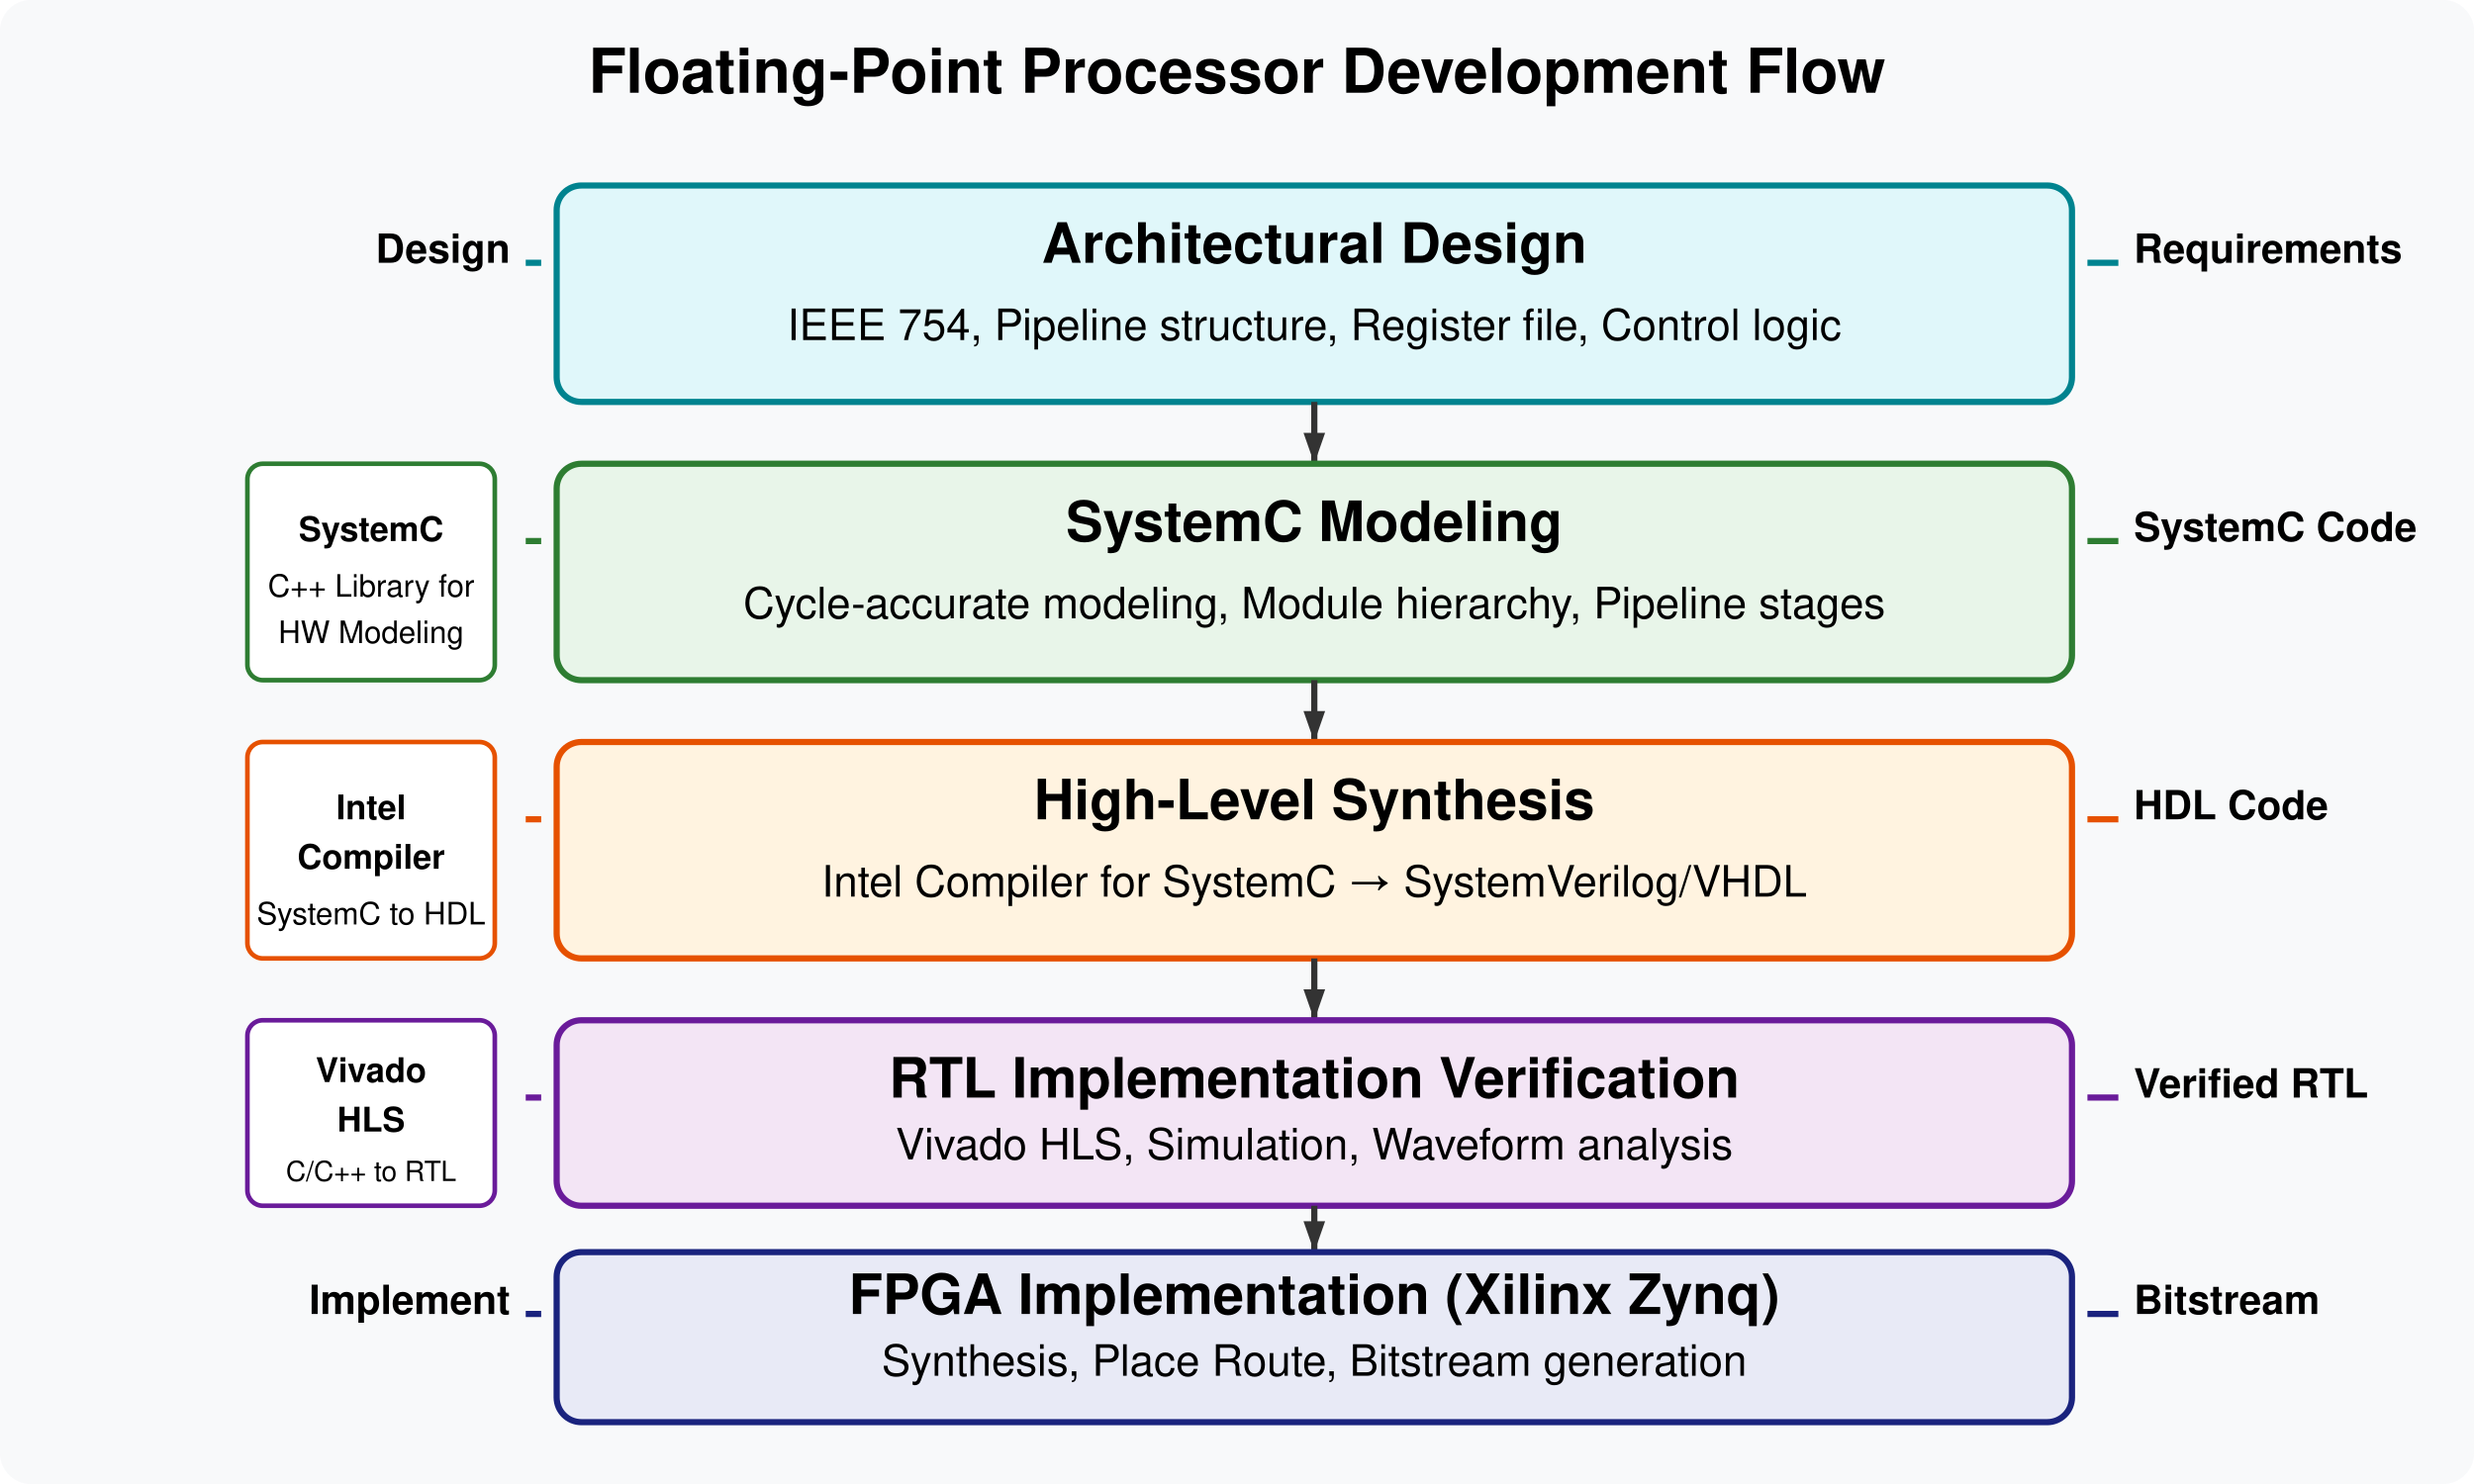
\includegraphics[width=0.8\textwidth]{figures/development.png}
\caption{Development flow stages of the pipelined floating-point processor}
\label{fig:top_level}
\end{figure}

\section{Design Requirements and Constraints}
\label{sec:design_req}

The floating-point processor design must satisfy the following functional requirements:

\begin{itemize}
\item Support for 32-bit single precision floating point format with 1 sign bit, 8 exponent bits, and 23 significand bits.
\item Implementation of addition, subtraction, multiplication and division operations with full precision.
\item Proper handling of special cases like zero, infinity, NaN and denormalised numbers.
\item Round to nearest (ties for even) to be implemented.
\item Handling exceptions like overflow, underflow, division by zero and invalid operations.
\end{itemize}

\section{IEEE 754 Floating-Point Standard}
\label{sec:ieee754_standard}

The IEEE 754 standard, formally known as IEEE Standard for Floating-Point Arithmetic, defines the technical details for floating-point computation. First published in 1985 and revised in 2008 (IEEE 754-2008), it has become the de facto standard for floating-point arithmetic in modern computing systems. This section provides a comprehensive overview of the standard's key aspects that directly influence the architectural design decisions of our pipelined floating-point processor.

\subsection{Standard Overview and Motivation}
\label{subsec:ieee754_overview}

Prior to IEEE 754, different computer manufacturers implemented floating-point arithmetic with varying formats, precision levels, and behavioral characteristics. This lack of standardization created significant portability issues for scientific and engineering applications. The IEEE 754 standard addresses these challenges by establishing:

\begin{itemize}
\item Standardized binary and decimal floating-point formats
\item Consistent rounding behaviors across different implementations
\item Uniform handling of special values and exceptional conditions
\item Predictable results for identical operations across different platforms
\end{itemize}

The standard ensures that floating-point operations produce identical results regardless of the underlying hardware implementation, provided both systems comply with IEEE 754 specifications.

\subsection{Floating-Point Number Representation}
\label{subsec:ieee754_representation}

IEEE 754 defines multiple precision formats, with single precision (binary32) being most relevant to our implementation. The mathematical representation of a floating-point number follows the formula:

$$(-1)^S \times (1 + M) \times 2^{E-bias}$$

Where:
\begin{itemize}
\item $S$ is the sign bit
\item $M$ is the significand (mantissa) representing the fractional part
\item $E$ is the stored exponent value
\item $bias$ is the exponent bias (127 for single precision)
\end{itemize}

\subsubsection{Single Precision Format (Binary32)}
\label{subsubsec:single_precision}

The 32-bit single precision format allocates bits as follows:

\begin{itemize}
\item \textbf{Bit 31:} Sign bit ($S$)
\item \textbf{Bits 30-23:} 8-bit exponent field ($E$)
\item \textbf{Bits 22-0:} 23-bit significand field ($M$)
\end{itemize}

The biased exponent representation allows for efficient comparison operations and eliminates the need for separate sign handling in the exponent. The bias value of 127 means that actual exponents range from -126 to +127, with stored values from 1 to 254 (0 and 255 are reserved for special cases).

\subsection{Special Values and Edge Cases}
\label{subsec:ieee754_special_values}

IEEE 754 defines specific encodings for special values that cannot be represented in the standard normalized format:

\subsubsection{Zero Values}
\label{subsubsec:zero_values}

Zero is represented with both exponent and significand fields set to zero. The standard defines both positive zero (+0) and negative zero (-0), distinguished only by the sign bit. These values are considered equal in comparisons but may produce different results in certain operations (e.g., division by zero).

\subsubsection{Denormalized Numbers (Subnormals)}
\label{subsubsec:denormalized}

When the exponent field is zero but the significand is non-zero, the value represents a denormalized number. These values use the formula:

$$(-1)^S \times (0 + M) \times 2^{1-bias}$$

Denormalized numbers provide gradual underflow, allowing representation of very small numbers that would otherwise underflow to zero. This feature maintains numerical stability in algorithms sensitive to small value precision.

\subsubsection{Infinity Values}
\label{subsubsec:infinity}

Infinity is represented with the exponent field set to all ones (255 for single precision) and the significand field set to zero. Like zero, infinity has both positive and negative variants. Infinity results from operations that exceed the representable range, such as division by zero or overflow conditions.

\subsubsection{Not-a-Number (NaN)}
\label{subsubsec:nan}

NaN values have the exponent field set to all ones and a non-zero significand. The standard defines two types of NaN:

\begin{itemize}
\item \textbf{Quiet NaN (qNaN):} Propagates through operations without raising exceptions
\item \textbf{Signaling NaN (sNaN):} Triggers an invalid operation exception when used in arithmetic operations
\end{itemize}

The most significant bit of the significand typically distinguishes between quiet and signaling NaN values.

\subsection{Rounding Modes}
\label{subsec:ieee754_rounding}

IEEE 754 defines five rounding modes to handle cases where the exact result cannot be represented in the target format:

\subsubsection{Round to Nearest, Ties to Even}
\label{subsubsec:round_nearest_even}

This is the default rounding mode, implemented in our processor design. When the result falls exactly between two representable values, rounding occurs toward the value with an even least significant bit. This approach eliminates systematic bias in repeated calculations.

\subsubsection{Round to Nearest, Ties Away from Zero}
\label{subsubsec:round_away_zero}

Similar to the previous mode, but ties are resolved by rounding away from zero rather than toward even values.

\subsubsection{Round Toward Zero (Truncation)}
\label{subsubsec:round_toward_zero}

Results are truncated toward zero, effectively discarding fractional portions. This mode never increases the magnitude of the result.

\subsubsection{Round Toward Positive Infinity}
\label{subsubsec:round_positive_infinity}

Results are always rounded toward positive infinity, useful in interval arithmetic applications.

\subsubsection{Round Toward Negative Infinity}
\label{subsubsec:round_negative_infinity}

Results are always rounded toward negative infinity, complementing the previous mode for interval arithmetic.

\subsection{Exception Handling}
\label{subsec:ieee754_exceptions}

IEEE 754 defines five types of floating-point exceptions that may occur during arithmetic operations:

\subsubsection{Invalid Operation}
\label{subsubsec:invalid_operation}

Occurs when an operation has no mathematically defined result, such as:
\begin{itemize}
\item Square root of a negative number
\item Addition of infinities with opposite signs
\item Multiplication of zero by infinity
\end{itemize}

The result is typically a NaN value.

\subsubsection{Division by Zero}
\label{subsubsec:division_by_zero}

Triggered when dividing a finite non-zero number by zero. The result is signed infinity.

\subsubsection{Overflow}
\label{subsubsec:overflow}

Occurs when the result magnitude exceeds the largest representable finite value. Depending on the rounding mode, the result may be infinity or the largest representable finite value.

\subsubsection{Underflow}
\label{subsubsec:underflow}

Happens when the result is too small to be represented as a normalized number. The result may be zero or a denormalized number, depending on the specific circumstances.

\subsubsection{Inexact}
\label{subsubsec:inexact}

Triggered when the result cannot be represented exactly and must be rounded. This is the most common exception in floating-point operations.

\subsection{IEEE 754 Compliance Requirements}
\label{subsec:ieee754_compliance}

For our processor to be IEEE 754 compliant, it must implement:

\begin{itemize}
\item Correct handling of all special values (zero, infinity, NaN, denormalized numbers)
\item Proper exception detection and reporting mechanisms
\item At least one required rounding mode (round to nearest, ties to even)
\item Consistent behavior for edge cases and boundary conditions
\item Correct sign handling for all operations and special cases
\end{itemize}

The architectural decisions in subsequent sections are designed to meet these compliance requirements while maintaining efficient FPGA implementation characteristics.

\section{Introduction to Architectural Design}
\label{sec:arch_intro}

This section describes the architectural design of a pipelined floating-point processor that balances IEEE 754 compliance with performance optimization and resource efficiency for Xilinx Zynq FPGA implementation. The design addresses pipeline hazards, ensures IEEE 754 compliant operations, and optimizes FPGA resources through critical components including exponent alignment, normalization, and rounding logic to achieve both accuracy and implementation efficiency \cite{ref16}.

\begin{figure}[h]
\centering
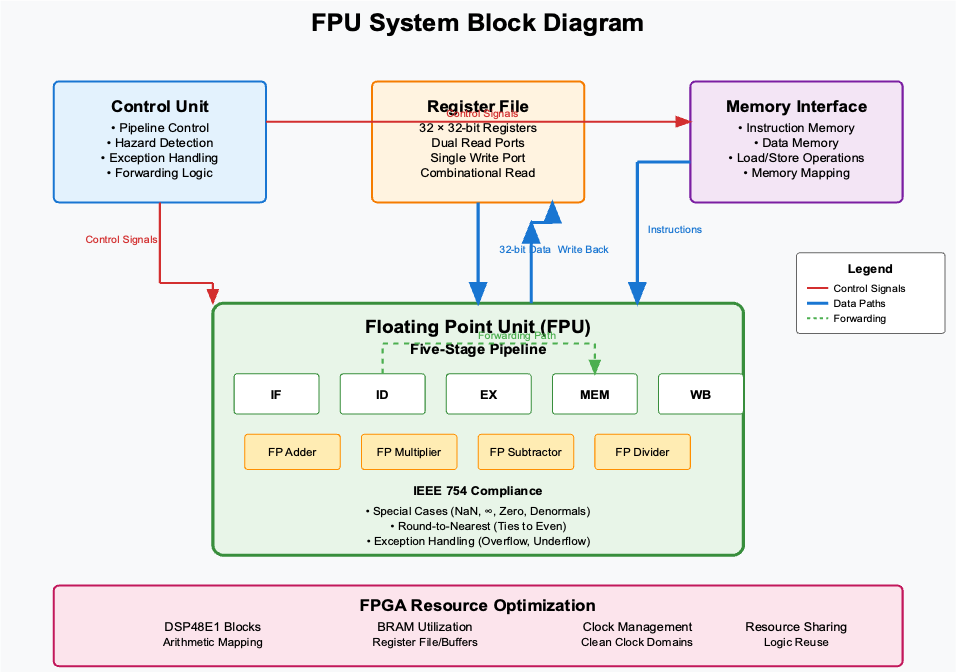
\includegraphics[width=0.8\textwidth]{figures/Con.png}
\caption{Control logic architecture of the pipelined floating-point processor}
\label{fig:control_logic}
\end{figure}

\subsection{Floating-Point Format and Representation}
\label{subsec:fp_format}

Building upon the IEEE 754 standard discussed in Section \ref{sec:ieee754_standard}, the processor implements the single-precision binary floating-point format with the following architectural considerations:

\begin{itemize}
\item \textbf{Sign Bit:} 1 bit indicating value sign (0 for positive, 1 for negative)
\item \textbf{Exponent:} 8 bits representing the biased exponent (actual exponent + 127)
\item \textbf{Significand:} 23 bits representing the fractional portion of the significand (with implicit leading 1 for normalized values)
\end{itemize}

Special values are encoded according to IEEE 754 conventions as detailed in Section \ref{subsec:ieee754_special_values}:

\begin{itemize}
\item \textbf{Zero:} Exponent = 0, Significand = 0 (signed)
\item \textbf{Denormalized Numbers:} Exponent = 0, Significand $\neq$ 0
\item \textbf{Infinity:} Exponent = 255, Significand = 0 (signed)
\item \textbf{NaN:} Exponent = 255, Significand $\neq$ 0
\end{itemize}

\subsection{Pipeline Structure}
\label{subsec:pipeline_structure}

The floating-point processor uses a five-stage pipeline architecture, based on the classic RISC-V pipeline structure modified for floating-point operations. The pipeline stages are:

\begin{enumerate}
\item \textbf{Instruction Fetch (IF):} Retrieves instruction from program memory
\item \textbf{Decode (ID):} Decodes instruction and reads operands from register file
\item \textbf{Execute (EX):} Performs floating-point operation (addition, subtraction, multiplication, division) with full IEEE 754 compliance
\item \textbf{Memory (MEM):} In this implementation, acts primarily as a pipeline register
\item \textbf{Writeback (WB):} Writes results back to register file
\end{enumerate}

This pipeline structure allows for efficient overlapping of instruction execution, with each stage processing a different instruction simultaneously, thereby maximizing throughput while maintaining precise IEEE 754 compliance as specified in Section \ref{subsec:ieee754_compliance}.

\subsection{Control Logic Design}
\label{subsec:control_logic}

The control logic is responsible for orchestrating all stages of the pipeline and for handling various hazards while ensuring IEEE 754 exception handling compliance:

\begin{itemize}
\item \textbf{Pipeline Stall Logic:} Helps pause the pipeline when required for multi-cycle operations or when hazards must be resolved
\item \textbf{Hazard Detection:} Operates to detect data hazards between instructions in the pipeline and determines the necessary handling routes
\item \textbf{Forwarding Logic:} Implements data forwarding to resolve data hazards without stalling the pipeline
\item \textbf{Exception Handling:} Detects and manages IEEE 754 exceptions (overflow, underflow, invalid operation, division by zero, and inexact) as defined in Section \ref{subsec:ieee754_exceptions}
\item \textbf{Special Value Detection:} Identifies and properly handles special IEEE 754 values during pipeline execution
\end{itemize}



\section{Register File Design}
\label{sec:register_file}

The register file is designed to support the IEEE 754 compliant floating-point operations:

\begin{itemize}
\item Support for 32 floating-point registers, each 32 bits wide for single-precision values
\item Dual read ports and single write port to maintain instruction throughput
\item Synchronous write operations on positive clock edge
\item Combinational read operations for minimal latency
\item Special value preservation through the register file to maintain IEEE 754 bit patterns
\end{itemize}

\section{Memory Interface}
\label{sec:memory_interface}

While this implementation focuses on floating-point processing pipelines rather than memory operations, the architecture includes:

\begin{itemize}
\item \textbf{Instruction Memory Interface:} For instruction fetching with proper IEEE 754 instruction encoding
\item \textbf{Data Memory Interface:} For loading and storing floating-point values while preserving IEEE 754 bit patterns
\item \textbf{Memory Mapping:} Appropriate address space allocation for floating-point data structures
\end{itemize}

\section{Design Considerations for FPGA Implementation}
\label{sec:fpga_considerations}

The architecture incorporates specific considerations for FPGA implementation while maintaining IEEE 754 compliance:

\begin{itemize}
\item \textbf{Efficient use of DSP blocks:} Arithmetic units are designed for effective mapping to DSP48E1 blocks while preserving IEEE 754 precision requirements
\item \textbf{Optimal memory resource utilization:} Register file and buffers are designed for efficient use of BRAM while maintaining IEEE 754 special value handling
\item \textbf{Pipeline depth optimization:} Pipeline depth is optimized to achieve target clock frequency while ensuring IEEE 754 operation completion
\item \textbf{Clock domain management:} Clean clock domain design with proper IEEE 754 exception propagation across domains
\item \textbf{Resource sharing:} Controlled resource sharing between operations requiring similar computations without compromising IEEE 754 compliance
\item \textbf{Special value optimization:} FPGA-optimized logic for detecting and handling IEEE 754 special values efficiently
\end{itemize}

The architectural decisions outlined in this chapter enable the SystemC implementation described in subsequent chapters to effectively map to both simulation environments and real-world FPGA hardware while maintaining full IEEE 754 standard compliance. The comprehensive IEEE 754 implementation ensures portability, predictability, and interoperability with other IEEE 754 compliant systems.
\chapter{SystemC Modelling and Implementation}
\label{chap:systemc_modelling}

\section{Introduction}

This chapter presents the comprehensive SystemC implementation of our pipelined floating-point processor, covering both the overall processor architecture and the detailed implementation of IEEE 754 floating-point arithmetic units. The implementation translates the architectural design into executable SystemC code that maintains IEEE 754 compliance while ensuring synthesis compatibility with Intel SystemC-to-SystemVerilog tools.

The key challenge addressed is maintaining IEEE 754 compliance while ensuring the SystemC code translates to efficient, synthesizable hardware. Our approach balances performance, area efficiency, and timing constraints through carefully designed pipeline architectures and optimized arithmetic units.

\section{SystemC Modelling Approach}
\label{sec:systemc_approach}

SystemC provides a C++ based hardware description and modelling language that bridges the gap between software and hardware design. As a class library built on standard C++, it extends the language with hardware constructs including:

\begin{itemize}
    \item \textbf{Modules:} Act as hardware building blocks that represent distinct parts of the system and hide internal details behind interfaces
    \item \textbf{Ports:} Define communication interfaces between modules
    \item \textbf{Signals:} Act as wires between modules carrying data from one port to another, mimicking hardware connections
    \item \textbf{Processes:} Independent workers inside modules that run simultaneously, triggered by signals, clocks or events
    \item \textbf{Events:} Help synchronize different parts of design, ensuring proper timing
    \item \textbf{Clocks:} Provide timing reference for synchronous logic with flip-flops, registers and state machines updating on clock edges
\end{itemize}

\subsection{Cycle-Accurate RTL Abstraction}
\label{subsec:cycle_accurate}

For this pipeline implementation, we employ a cycle-accurate RTL-like abstraction level that models the behavior of our processor where every clock cycle matters, and pipeline stages are modelled precisely. This approach allows us to:

\begin{itemize}
    \item Observe how instructions flow through the pipeline
    \item Model data dependencies and control flow logic accurately
    \item Verify functional correctness with exact timing and no approximations
    \item Generate synthesizable RTL that directly maps to hardware
\end{itemize}

The model behaves like Verilog/VHDL making actual chip design straightforward. While higher abstraction levels could improve simulation speed, the cycle-accurate approach was necessary to validate our processor architecture and ensure synthesis compatibility.

\section{SystemC Synthesis Constraints and Design Methodology}
\label{sec:synthesis_constraints}

The Intel SystemC compiler imposes specific requirements for synthesizable code that influenced our entire design methodology:

\begin{itemize}
    \item \textbf{Thread Structure}: Use \texttt{SC\_CTHREAD} instead of \texttt{SC\_METHOD} for clocked processes
    \item \textbf{State Management}: Explicit state transitions with \texttt{while(true)} loops and \texttt{wait()} statements
    \item \textbf{Reset Handling}: Automatic reset using \texttt{reset\_signal\_is()} declarations
    \item \textbf{Data Types}: Only synthesizable types (\texttt{sc\_uint}, \texttt{bool}) - no floating-point types
    \item \textbf{Pipeline Registers}: Explicit pipeline stage separation with proper timing
\end{itemize}

Each \texttt{wait()} statement corresponds to a clock boundary, and code between consecutive \texttt{wait()} statements represents combinational logic within a single clock cycle.

\section{SystemC Module Hierarchy}
\label{sec:module_hierarchy}

Our SystemC implementation follows a hierarchical structure combining the five-stage pipeline with specialized IEEE 754 arithmetic units. The processor implementation consists of the following primary modules:

\begin{itemize}
    \item \textbf{Instruction Fetch Unit}: Program counter management and instruction memory access
    \item \textbf{Decode Unit}: Instruction decoding and register file access
    \item \textbf{Execute Unit}: Floating-point operation execution with dedicated arithmetic units
    \item \textbf{Memory Access Unit}: Pipeline register stage for memory operations
    \item \textbf{Writeback Unit}: Result integration into processor state
    \item \textbf{Arithmetic Units}: IEEE 754 compliant adder, subtractor, multiplier, and divider
    \item \textbf{Supporting Components}: Instruction memory and register file
\end{itemize}

Each stage connects to the next through registers and ports, forming the complete processor data path. Each process typically has two main sections: a reset section for initialization and an infinite loop where communication and computation occur.

\begin{figure}[htbp]
    \centering
    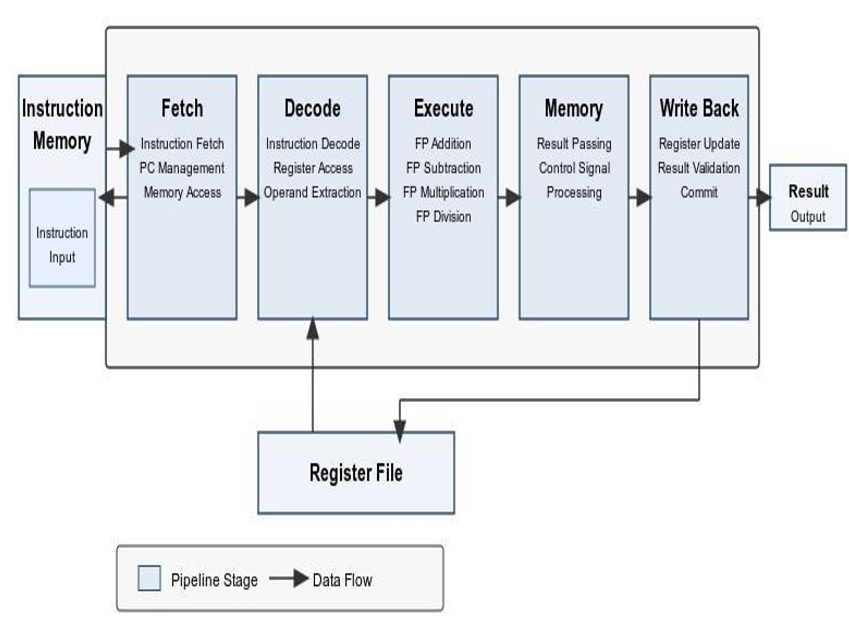
\includegraphics[width=0.8\textwidth]{pipeline_diagram.png}
    \caption{SystemC module hierarchy of the pipelined floating-point processor}
    \label{fig:systemc_hierarchy}
\end{figure}



\section{Interface Definitions and Communication}
\label{sec:interface_definitions}

Each module defines clear interfaces using SystemC ports and signals. The primary pipeline interface includes:

\begin{lstlisting}[caption={Pipeline Stage Interface}]
// Input ports
sc_in<bool> clk;                    // System clock
sc_in<bool> reset;                  // Active-high reset
sc_in<bool> stall;                  // Stall signal
sc_in<sc_uint<32>> instruction_in;  // Instruction input
sc_in<bool> valid_in;               // Validity flag for input

// Output ports
sc_out<sc_uint<32>> result_out;     // Operation result
sc_out<sc_uint<5>> rd_out;          // Destination register
sc_out<bool> reg_write_out;         // Register write enable
sc_out<bool> valid_out;             // Validity flag for output
sc_out<sc_uint<32>> instruction_out; // Instruction forwarded
\end{lstlisting}

These standardized interfaces ensure consistent communication between pipeline stages, facilitating modular design and verification.

\section{IEEE 754 Arithmetic Units Implementation}
\label{sec:arithmetic_units}

The heart of our floating-point processor lies in the IEEE 754 compliant arithmetic units. Each unit follows synthesis-compatible design patterns while maintaining full standard compliance.

\subsection{IEEE 754 Addition/Subtraction Algorithm}
\label{subsec:ieee754_addition}

\subsubsection{Algorithm Overview}

IEEE 754 addition/subtraction follows these steps:
\begin{enumerate}
    \item Extract sign, exponent, and mantissa from both operands
    \item Align mantissas by shifting the smaller operand
    \item Perform mantissa addition or subtraction based on signs
    \item Normalize the result and handle overflow/underflow
\end{enumerate}

\subsubsection{3-Stage Implementation}

The addition/subtraction unit implements a 3-stage process optimized for synthesis compatibility:

\textbf{Stage 1: Operand Extraction}
\begin{lstlisting}[caption=Extraction Stage Implementation]
void extract_stage() {
    // Reset outputs
    sign_a_reg2.write(0);
    // ... other resets
    wait();
    
    while (true) {
        // Extract IEEE 754 components
        bool sign_a = A_reg1.read()[31];
        sc_uint<8> exp_a = A_reg1.read().range(30, 23);
        sc_uint<24> mant_a;
        
        if (exp_a == 0) {
            mant_a = (sc_uint<24>)((sc_uint<1>(0), 
                     A_reg1.read().range(22, 0)));
        } else {
            mant_a = (sc_uint<24>)((sc_uint<1>(1), 
                     A_reg1.read().range(22, 0)));
        }
        
        // Register for next stage
        sign_a_reg2.write(sign_a);
        exp_a_reg2.write(exp_a);
        mant_a_reg2.write(mant_a);
        wait();
    }
}
\end{lstlisting}

\textbf{Stage 2: Addition/Subtraction Logic}
\begin{lstlisting}[caption=Addition Core Logic]
void add_stage() {
    // Reset state
    wait();
    
    while (true) {
        // Determine larger operand for alignment
        if (exp_a_reg2.read() > exp_b_reg2.read()) {
            diff = exp_a_reg2.read() - exp_b_reg2.read();
            tmp_mantissa = mant_b_reg2.read() >> diff;
            
            if (sign_a_reg2.read() == sign_b_reg2.read()) {
                // Same signs: addition
                out_mantissa = mant_a_reg2.read() + tmp_mantissa;
            } else {
                // Different signs: subtraction
                out_mantissa = mant_a_reg2.read() - tmp_mantissa;
            }
        }
        // Handle other cases...
        wait();
    }
}
\end{lstlisting}

\textbf{Stage 3: Normalization}
\begin{lstlisting}[caption=Normalization Stage]
void normalize_stage() {
    O.write(0);
    wait();
    
    while (true) {
        if (norm_mantissa[24]) {
            // Overflow: shift right, increment exponent
            norm_exponent = norm_exponent + 1;
            norm_mantissa = norm_mantissa >> 1;
        } else if (norm_mantissa[23] == 0) {
            // Underflow: count leading zeros, shift left
            for (lz = 0; lz < 24 && norm_mantissa[23-lz] == 0; lz++);
            norm_exponent = norm_exponent - lz;
            norm_mantissa = norm_mantissa << lz;
        }
        
        result = (sign, norm_exponent, norm_mantissa.range(22,0));
        O.write(result);
        wait();
    }
}
\end{lstlisting}

\subsection{IEEE 754 Multiplication Algorithm}
\label{subsec:ieee754_multiplication}

\subsubsection{Algorithm Design}

Multiplication requires additional stages due to the complexity of 24×24-bit mantissa multiplication.

The key algorithmic steps include:
\begin{enumerate}
    \item \textbf{Operand Preparation}: Extract components and handle special cases (NaN, infinity, zero)
    \item \textbf{Sign Calculation}: XOR operation on sign bits  
    \item \textbf{Exponent Addition}: Add biased exponents and adjust for bias
    \item \textbf{Mantissa Multiplication}: 24×24 bit multiplication including implicit leading ones
    \item \textbf{Normalization \& Rounding}: Final result adjustment with IEEE 754 compliance
\end{enumerate}
\begin{lstlisting}[caption=Multiplication and Exponent Addition]
void mult_cycle2_exp_stage() {
    wait(); // Reset state
    
    while (true) {
        // Complete 24x24 bit multiplication
        sc_uint<48> full_mult_result = 
            mant_a_reg3.read() * mant_b_reg3.read();
        
        // Calculate result sign (XOR)
        bool result_sign = sign_a_reg3.read() ^ sign_b_reg3.read();
        
        // Add exponents and subtract bias
        sc_uint<9> temp_exp = exp_a_reg3.read() + exp_b_reg3.read();
        sc_uint<9> result_exp = (temp_exp >= 127) ? 
                                temp_exp - 127 : 0;
        
        result_sign_reg4.write(result_sign);
        result_exp_reg4.write(result_exp);
        mult_result_reg4.write(full_mult_result);
        wait();
    }
}
\end{lstlisting}

\textbf{Stage 5: Normalization \& Rounding}
\begin{lstlisting}[caption=Multiplication Normalization]
void normalize_round_stage() {
    O.write(0);
    wait();
    
    while (true) {
        sc_uint<48> mult_result = mult_result_reg4.read();
        
        // Normalization based on result magnitude
        if (mult_result[47]) {
            // Result is 1.xxx (overflow)
            final_mantissa = mult_result.range(46, 24);
            final_exponent = exp_result + 1;
        } else if (mult_result[46]) {
            // Result is 0.1xxx (normal)
            final_mantissa = mult_result.range(45, 23);
            final_exponent = exp_result;
        } else {
            // Underflow: find first significant bit
            // Shift left and adjust exponent accordingly
        }
        
        result = (sign_result, final_exponent, final_mantissa);
        O.write(result);
        wait();
    }
}
\end{lstlisting}

\subsection{IEEE 754 Division Algorithm}
\label{subsec:ieee754_division}

\subsubsection{Algorithm for Iterative Division}

Division is the most complex operation, requiring an iterative division algorithm. The key algorithmic steps include:

\begin{enumerate}
    \item \textbf{Preparation}: Input validation and special case handling
    \item \textbf{Sign Determination}: XOR operation on operand signs
    \item \textbf{Exponent Subtraction}: Subtract divisor exponent from dividend exponent
    \item \textbf{Iterative Division}: Restoring division algorithm for significands
    \item \textbf{Normalization}: Final result formatting with exception detection
\end{enumerate}

\textbf{Division Iteration Implementation:}
\begin{lstlisting}[caption=Division Iteration Stage]
void division_stage1() {
    // Reset state
    wait();
    
    while (true) {
        sc_uint<32> x_val = x_val_reg2.read();
        sc_uint<32> y_val = y_val_reg2.read();
        sc_uint<32> r = 0;

        // Perform 5 division iterations per stage
        for (sc_uint<3> i = 0; i < 5; i++) {
            r = r << 1;
            if (x_val >= y_val) {
                x_val = x_val - y_val;
                r = r | 1;
            }
            x_val = x_val << 1;
        }

        // Pass results to next stage
        x_val_reg3.write(x_val);
        r_reg3.write(r);
        wait();
    }
}
\end{lstlisting}



\section{Processor Pipeline Implementation}
\label{sec:processor_pipeline}

\subsection{Instruction Fetch Stage}
\label{subsec:instruction_fetch}

The instruction fetch stage is the first stage of our five-stage pipeline and is responsible for reading instructions from memory and providing them to the decode stage. Our SystemC implementation maintains a Program Counter (PC) register that tracks the address of the next instruction to be fetched and includes comprehensive instruction validity checking.

Key functionality includes:
\begin{enumerate}
    \item \textbf{Program Counter Management}: Maintains and increments the PC register for sequential instruction execution
    \item \textbf{Instruction Memory Access}: Interfaces with instruction memory using address signals
    \item \textbf{Instruction Validity Checking}: Validates fetched instructions and handles termination conditions
    \item \textbf{Stall Handling}: Supports pipeline stall mechanisms for hazard resolution
    \item \textbf{Termination Detection}: Recognizes end-of-program conditions through zero instruction detection
\end{enumerate}

The instruction fetch process operates synchronously with the system clock and includes reset handling for proper initialization. When a stall condition is not active, the stage fetches the instruction from memory at the current PC address, validates the instruction, and prepares it for the decode stage. The PC is incremented by 4 bytes (32 bits) for the next instruction fetch, following standard RISC architecture conventions.

\begin{lstlisting}[caption={Instruction Fetch Process}]
// Instruction fetch process
void ifu_process() {
    if (reset) {
        pc = 0;
        terminated = false;
        ifu_instruction_out = 0;
        ifu_valid_out = false;
    } else if (!internal_stall && !terminated) {
        sc_uint<32> current_pc = pc;
        imem_address = current_pc;
        sc_uint<32> instruction = imem_instruction;
        
        ifu_instruction_out = instruction;
        ifu_valid_out = (instruction != 0);
        pc_out = current_pc;
        
        if (instruction == 0) {
            terminated = true;
            ifu_valid_out = false;
        } else {
            pc = current_pc + 4;
        }
    }
}
\end{lstlisting}

The fetch stage interfaces with the instruction memory through the \texttt{imem\_address} output port and receives instruction data through the \texttt{imem\_instruction} input port. The \texttt{terminated} flag prevents further instruction fetching when the end of the program is reached, indicated by a zero instruction value.

\subsection{Decode Stage}
\label{subsec:decode_stage}

The decode stage is the second stage of the pipeline and is responsible for interpreting the fetched instruction and extracting the necessary operands and control signals. This stage performs the critical task of translating the 32-bit instruction word into meaningful control and data signals for the subsequent execute stage.

The decode stage performs several essential functions:
\begin{enumerate}
    \item \textbf{Instruction Field Extraction}: Decodes the instruction format to extract source and destination register addresses
    \item \textbf{Register File Access}: Reads operand values from the register file using extracted register addresses
    \item \textbf{Control Signal Generation}: Generates control signals such as register write enable
    \item \textbf{Instruction Forwarding}: Passes the instruction to subsequent pipeline stages for continued processing
    \item \textbf{Validity Propagation}: Maintains instruction validity signals throughout the pipeline
\end{enumerate}

The instruction decoding follows a standard RISC instruction format where source registers rs1 and rs2 are located at specific bit positions within the instruction word. The destination register rd is also extracted from its designated bit field. The register file provides the actual operand values that will be used in the execute stage for floating-point operations.

\begin{lstlisting}[caption={Decode Process}]
void decode_process() {
    if (reset) {
        op1_out = 0;
        op2_out = 0;
        rd_out = 0;
        reg_write_out = false;
        decode_valid_out = false;
        decode_instruction_out = 0;
    } else if (!internal_stall) {
        decode_valid_out = ifu_valid_out;
        decode_instruction_out = ifu_instruction_out;
        if (ifu_valid_out && ifu_instruction_out != 0) {
            sc_uint<5> rs1 = (ifu_instruction_out >> 15) & 0x1F;
            sc_uint<5> rs2 = (ifu_instruction_out >> 20) & 0x1F;
            sc_uint<5> rd = (ifu_instruction_out >> 7) & 0x1F;
            op1_out = reg_file[rs1];
            op2_out = reg_file[rs2];
            rd_out = rd;
            reg_write_out = true;
        } else {
            op1_out = 0;
            op2_out = 0;
            rd_out = 0;
            reg_write_out = false;
        }
    }
}
\end{lstlisting}

The decode stage maintains careful synchronization with the fetch stage through validity signals and handles stall conditions by preserving the current state until the stall is released. The extracted operands and control signals are forwarded to the execute stage for arithmetic processing.

\subsection{Execute Stage}
\label{subsec:execute_stage}

The execute stage is the computational heart of the floating-point processor pipeline, where the actual IEEE 754 floating-point operations are performed. This stage integrates all four arithmetic units (addition, subtraction, multiplication, and division) and selects the appropriate operation based on the instruction opcode.

The execute stage performs the following critical functions:
\begin{enumerate}
    \item \textbf{Operation Selection}: Decodes the instruction opcode to determine which floating-point operation to perform
    \item \textbf{Arithmetic Unit Integration}: Interfaces with the IEEE 754 compliant arithmetic units for computation
    \item \textbf{Result Generation}: Produces the floating-point operation result in IEEE 754 format
    \item \textbf{Exception Handling}: Manages floating-point exceptions and special cases
    \item \textbf{Control Flow Management}: Handles pipeline control signals and instruction forwarding
\end{enumerate}

The execute stage operates with multiple arithmetic units running in parallel, allowing for concurrent execution of different instruction types. The opcode field of the instruction determines which arithmetic unit's result is selected for output. This design enables efficient utilization of hardware resources while maintaining the simplicity of the pipeline control logic.

\begin{lstlisting}[caption={Execute Process}]
// Execute process
void execute_process() {
    if (reset) {
        result_out = 0;
        rd_out = 0;
        reg_write_out = false;
        valid_out = false;
        instruction_out = 0;
    } else if (!stall) {
        valid_out = valid_in;
        rd_out = rd_in;
        reg_write_out = reg_write_in;
        instruction_out = instruction_in;
        
        if (valid_in && reg_write_in) {
            switch (opcode) {
                case 0x00: result_out = fp_add_result; break;    // Addition
                case 0x04: result_out = fp_sub_result; break;    // Subtraction  
                case 0x08: result_out = fp_mul_result; break;    // Multiplication
                case 0x0C: result_out = fp_div_result; break;    // Division
                default:   result_out = 0; break;
            }
        }
    }
}
\end{lstlisting}

The switch statement implementation provides a clean and efficient method for operation selection, with each arithmetic unit producing its result independently. The execute stage ensures that only valid instructions with proper register write enable signals produce meaningful results, maintaining the integrity of the pipeline operation.

\subsection{Memory and Writeback Stages}
\label{subsec:memory_writeback}

The memory and writeback stages complete the five-stage pipeline by handling data storage operations and updating the processor's architectural state. In our floating-point processor implementation, the memory stage primarily serves as a pipeline register since the focus is on computational operations rather than memory access.

\subsubsection{Memory Stage Functionality}

The memory stage serves several important purposes in the pipeline:
\begin{enumerate}
    \item \textbf{Pipeline Register Function}: Maintains pipeline timing and provides buffer between execute and writeback stages
    \item \textbf{Signal Propagation}: Forwards results and control signals from execute stage to writeback stage
    \item \textbf{Timing Isolation}: Provides additional clock cycle for complex memory operations if needed in future extensions
    \item \textbf{Stall Support}: Integrates with pipeline stall mechanism for hazard handling
\end{enumerate}

\subsubsection{Writeback Stage Functionality}

The writeback stage is the final stage of the pipeline and is responsible for:
\begin{enumerate}
    \item \textbf{Register File Updates}: Controls the writing of computation results back to the register file
    \item \textbf{Result Validation}: Ensures only valid results from legitimate instructions are written
    \item \textbf{Instruction Completion}: Marks the completion of instruction execution cycle
    \item \textbf{Pipeline State Management}: Manages the final pipeline state and prepares for next instruction
\end{enumerate}

The writeback stage implements careful control logic to ensure that only valid instructions with proper write enable signals update the architectural state. This prevents corruption of the register file from invalid or cancelled instructions.

\begin{lstlisting}[caption={Memory and Writeback Processes}]
// Memory process
void memory_process() {
    if (!reset && !stall) {
        result_out = result_in;
        rd_out = rd_in;
        reg_write_out = reg_write_in;
        valid_out = valid_in;
        instruction_out = instruction_in;
    }
}

// Writeback process
void writeback_process() {
    if (!reset && !stall) {
        result_out = result_in;
        rd_out = rd_in;
        bool do_write = reg_write_in && valid_in && (instruction_in != 0);
        reg_write_en = do_write;
        valid_out = valid_in;
    }
}
\end{lstlisting}

The writeback logic includes a compound condition \texttt{do\_write} that ensures register writes only occur for valid, non-zero instructions with proper write enable signals. This multi-level validation prevents erroneous updates to the processor state and maintains the integrity of the floating-point computation results.


% SystemC to RTL Translation chapter for thesis
% This file will be included via % SystemC to RTL Translation chapter for thesis
% This file will be included via % SystemC to RTL Translation chapter for thesis
% This file will be included via \input{rtl_translation} in main thesis.tex

\chapter{High-Level Synthesis and RTL Generation}
\label{chap:rtl_translation}

\section{Introduction to High-Level Synthesis}
\label{sec:hls_introduction}

High-Level Synthesis (HLS) represents a paradigm shift in digital design methodology, enabling designers to describe hardware functionality using high-level programming languages rather than traditional Register Transfer Level (RTL) descriptions. This approach significantly accelerates the design process while maintaining the precision and control necessary for efficient hardware implementation. Our floating-point processor implementation leverages the Intel Compiler for SystemC (ICSC) to bridge the gap between algorithmic description and synthesizable hardware, providing both productivity benefits and design verification capabilities.

\section{Intel Compiler for SystemC Architecture}
\label{sec:icsc_architecture}

\subsection{Compiler Overview and Capabilities}
\label{subsec:icsc_overview}

The Intel Compiler for SystemC (version 1.6.13) represents a sophisticated translation framework that converts synthesizable SystemC designs into synthesizable SystemVerilog implementations. Built upon the robust Clang/LLVM 18.1.8 infrastructure and incorporating SystemC 3.0.0, ICSC provides a comprehensive solution for modern hardware design workflows.

The compiler architecture encompasses several key components that work together to ensure accurate and efficient translation:

\begin{itemize}
\item \textbf{Frontend Parser:} Based on Clang, providing complete C++11/14/17/20 support for parsing SystemC source code
\item \textbf{Elaboration Engine:} Handles SystemC-specific elaboration phase processing, including module hierarchy construction and signal binding
\item \textbf{Analysis Framework:} Performs synthesis-oriented analysis to detect non-synthesizable constructs and common coding mistakes
\item \textbf{Code Generation Backend:} Produces human-readable SystemVerilog (IEEE 1800-2017) compliant output
\item \textbf{Optimization Interface:} Maintains compatibility with downstream logic synthesis tools for further optimization
\end{itemize}

\subsection{SystemC Synthesizable Subset Support}
\label{subsec:systemc_subset}

ICSC supports a carefully defined synthesizable subset of SystemC that maps efficiently to hardware implementations. This subset includes:

\subsubsection{Process Support}
\label{subsubsec:process_support}

The compiler handles both method and thread processes with specific translation strategies:

\begin{itemize}
\item \textbf{SC\_METHOD:} Translated to combinational always\_comb blocks for purely combinational logic
\item \textbf{SC\_CTHREAD:} Converted to sequential always\_ff blocks for clocked sequential logic
\item \textbf{Sensitivity Lists:} Properly interpreted to generate appropriate trigger conditions in SystemVerilog
\end{itemize}

\subsubsection{Data Type Mapping}
\label{subsubsec:data_type_mapping}

SystemC data types are systematically mapped to their SystemVerilog equivalents:

\begin{itemize}
\item \textbf{sc\_uint<N>, sc\_int<N>:} Mapped to logic [N-1:0] and signed logic [N-1:0] respectively
\item \textbf{sc\_bv<N>, sc\_lv<N>:} Translated to logic [N-1:0] with appropriate value handling
\item \textbf{bool:} Directly mapped to SystemVerilog logic type
\item \textbf{Custom structs:} Preserved as SystemVerilog packed structures when synthesizable
\end{itemize}

\subsubsection{Communication Mechanisms}
\label{subsubsec:communication_mechanisms}

SystemC communication constructs are translated while preserving their intended hardware semantics:

\begin{itemize}
\item \textbf{sc\_signal:} Converted to appropriate wire or reg declarations based on driving context
\item \textbf{sc\_port/sc\_export:} Mapped to module interface ports with proper direction specification
\item \textbf{Hierarchical signals:} Maintained through proper signal routing in the generated hierarchy
\end{itemize}

\subsection{Translation Process Workflow}
\label{subsec:translation_workflow}

The ICSC translation process follows a systematic workflow designed to maintain design integrity while optimizing for synthesis:

\begin{enumerate}
\item \textbf{Source Analysis:} Clang frontend parses SystemC source files and builds an abstract syntax tree (AST)
\item \textbf{SystemC Elaboration:} The elaboration engine processes SystemC-specific constructs, resolving module hierarchy and signal connectivity
\item \textbf{Synthesis Checking:} Analysis passes identify non-synthesizable constructs and report potential issues
\item \textbf{Intermediate Representation:} Code is transformed into an intermediate representation suitable for hardware generation
\item \textbf{SystemVerilog Generation:} The backend generates human-readable SystemVerilog code with preserved design structure
\item \textbf{Optimization Interface:} Generated code is structured for efficient processing by downstream synthesis tools
\end{enumerate}

\section{Design Implementation with ICSC}
\label{sec:design_implementation}

\subsection{ICSC Project Setup and Compilation}
\label{subsec:icsc_project_setup}

To implement a custom design using ICSC, the process involves creating a proper CMake configuration and following the ICSC workflow. The floating-point processor project is placed in the ICSC designs directory and follows the standard ICSC project template structure.

\subsubsection{Project Template Configuration}
\label{subsubsec:project_template}

ICSC projects require a specific CMakeLists.txt configuration that utilizes the \texttt{svc\_target} function for SystemVerilog generation. The CMakeLists.txt file defines the project structure and compilation parameters:

\begin{lstlisting}[caption={ICSC Project CMakeLists.txt Configuration},label=lst:icsc_cmake]
# Design template CMakeList.txt file
project(mydesign)

# All synthesizable source files must be listed here (not in libraries)
add_executable(mydesign example.cpp)

# Test source directory
target_include_directories(mydesign PUBLIC $ENV{ICSC_HOME}/examples/template)

# Add compilation options
# target_compile_definitions(mydesign PUBLIC -DMYOPTION)
# target_compile_options(mydesign PUBLIC -Wall)

# Add optional library, do not add SystemC library (it added by svc_target)
#target_link_libraries(mydesign sometestbenchlibrary)

# svc_target will create @mydesign_sctool executable that runs code generation 
# and @mydesign that runs general SystemC simulation
# ELAB_TOP parameter accepts hierarchical name of DUT  
# (that is SystemC name, returned by sc_object::name() method)
svc_target(mydesign ELAB_TOP tb.dut_inst)
\end{lstlisting}

The \texttt{svc\_target} function is a CMake function defined in \linebreak
\texttt{\$ICSC\_HOME/lib64/cmake/SVC/svc\_target.cmake} that creates two executables: one for SystemVerilog generation and another for SystemC simulation.

\subsubsection{Project Directory Structure}
\label{subsubsec:project_directory}

The custom design should be placed in the \texttt{\$ICSC\_HOME/designs} folder. For our floating-point processor implementation, the project structure follows:

\begin{lstlisting}[caption={ICSC Project Directory Structure},label=lst:icsc_project_structure]
$ICSC_HOME/designs/my_project/
|-- CMakeLists.txt          # Project CMake configuration
|-- example.cpp             # Main SystemC implementation
|-- dut.h                   # Design under test header
`-- build/                  # Build directory (created during compilation)
    `-- sv_out/             # Generated SystemVerilog output
        `-- mydesign.sv     # Generated SystemVerilog file
\end{lstlisting}

\subsubsection{Compilation and Execution Workflow}
\label{subsubsec:compilation_workflow}

The complete workflow for compiling and executing the ICSC design follows these steps:

\begin{lstlisting}[caption={ICSC Compilation and Execution},label=lst:icsc_workflow]
# Navigate to ICSC installation directory
$ cd $ICSC_HOME

# Set up environment variables
$ source setenv.sh

# Create build directory
$ mkdir build && cd build

# Configure project with CMake
$ cmake ../                          # prepare Makefiles in Release mode

# Compile SystemC simulation for the design
$ make mydesign                      # compile SystemC simulation

# Navigate to design directory to run simulation
$ cd designs/my_project

# Execute SystemC simulation
$ ./mydesign                         # run SystemC simulation

# Generate SystemVerilog using svc_target
$ make mydesign_sctool              # runs SystemVerilog generation

# Examine generated SystemVerilog output
$ ls build/sv_out/
$ cat build/sv_out/mydesign.sv
\end{lstlisting}

The \texttt{svc\_target} function automatically handles the SystemVerilog generation process, creating the output in the \texttt{sv\_out} directory within the build folder. This approach ensures that both SystemC simulation and SystemVerilog generation are managed through the same CMake-based workflow, facilitating consistent development and verification processes.

\section{Intel Compiler for SystemC Implementation Details}
\label{sec:icsc_implementation}

\subsection{Compilation Framework Architecture}
\label{subsec:compilation_framework}

The Intel Compiler for SystemC operates as a sophisticated source-to-source translator built on proven compiler infrastructure. The framework leverages Clang/LLVM's robust parsing and analysis capabilities while adding SystemC-specific processing layers.

\subsubsection{Frontend Processing}
\label{subsubsec:frontend_processing}

The frontend processing stage handles the initial parsing and analysis of SystemC source code:

\begin{itemize}
\item \textbf{Lexical Analysis:} Tokenization of SystemC source files with recognition of SystemC-specific keywords and constructs
\item \textbf{Syntactic Analysis:} Construction of Abstract Syntax Tree (AST) preserving SystemC structural information
\item \textbf{Semantic Analysis:} Type checking and symbol resolution with SystemC type system awareness
\item \textbf{Elaboration Processing:} Handling of SystemC elaboration phase constructs including module instantiation and binding
\end{itemize}

\subsubsection{Intermediate Representation}
\label{subsubsec:intermediate_representation}

ICSC employs a specialized intermediate representation optimized for hardware synthesis:

\begin{itemize}
\item \textbf{Control Flow Representation:} Explicit modeling of sequential and combinational logic paths
\item \textbf{Data Path Analysis:} Identification of data dependencies and signal routing requirements
\item \textbf{Timing Model:} Preservation of SystemC timing semantics for accurate RTL generation
\item \textbf{Resource Mapping:} Preparation for efficient mapping to FPGA and ASIC resources
\end{itemize}

\subsection{SystemVerilog Code Generation}
\label{subsec:systemverilog_generation}

The code generation backend produces human-readable SystemVerilog that maintains the structural clarity of the original SystemC design while ensuring synthesis compatibility.

\subsubsection{Module Generation Strategy}
\label{subsubsec:module_generation}

Each SystemC module is translated to a corresponding SystemVerilog module with preserved hierarchy and connectivity:

\begin{lstlisting}[caption={Module Translation Example},label=lst:module_translation]
// Generated SystemVerilog from SystemC SC_MODULE
module FPProcessor (
    input logic clk,
    input logic reset,
    input logic stall,
    input logic [31:0] instruction_in,
    output logic [31:0] result_out,
    output logic result_valid,
    output logic [4:0] exception_flags
);

// Internal signal declarations preserved from SystemC
logic [31:0] if_id_instruction;
logic [31:0] id_ex_instruction;
logic [31:0] ex_mem_result;
logic [4:0] internal_exception_flags;

// Combinational logic from SC_METHOD processes
always_comb begin : decode_logic
    // Logic translated from SystemC SC_METHOD
end

// Sequential logic from SC_CTHREAD processes  
always_ff @(posedge clk) begin : pipeline_advance
    if (reset) begin
    end else begin
        // Normal operation logic from SystemC wait() loops
    end
end

ieee754_adder adder_inst (
    .clk(clk),
    .reset(reset),
    .operand_a(operand_a),
    .operand_b(operand_b),
    .result(add_result));

\end{lstlisting}

\subsubsection{Process Translation Methodology}
\label{subsubsec:process_translation}

SystemC processes are systematically converted to appropriate SystemVerilog constructs:

\begin{itemize}
\item \textbf{SC\_METHOD to always\_comb:} Combinational processes become always\_comb blocks with sensitivity lists derived from SystemC sensitivity
\item \textbf{SC\_CTHREAD to always\_ff:} Clocked thread processes become always\_ff blocks with proper clock and reset handling
\item \textbf{Sensitivity List Preservation:} SystemC sensitivity lists are accurately translated to SystemVerilog trigger conditions
\item \textbf{Wait Statement Handling:} SystemC wait() statements are converted to appropriate clock edge dependencies
\end{itemize}

\section{SystemC to Verilog Translation}
\label{sec:systemc_to_verilog}

The SystemC implementation was designed with synthesis in mind following these key guidelines:

\begin{itemize}
    \item \textbf{Synthesizable constructs:} Using only SystemC features that have clear hardware equivalents like avoiding dynamic memory allocation using fixed sized datatypes and using the write input states for all modules.
    
    \item \textbf{Explicit clocking:} All sequential logic triggered on a well-defined clock edge with no gated clocks or asynchronous resets \cite{ref13}.
    
    \item \textbf{Resource Aware Modeling:} FPGAs have finite logic elements, memory blocks and DSP slices considering trade-offs between efficient use of block vs distributed RAM for storage. By keeping FPGA resources in mind early in the modeling phase we avoid costly redesigns.
    
    \item \textbf{Bit-accurate modeling:} Every signal has defined bit widths and no unexpected conversions that could lead to extension or truncation during overflow and underflow rounding cases.
    
    \item \textbf{Combinational vs Sequential logic:} Combinatorial logic has no internal state and outputs purely dependent on inputs while sequential logic has stateful elements like registers that update on clock edges \cite{ref17}. This prevents unintended latches during synthesis.
\end{itemize}

 in main thesis.tex

\chapter{High-Level Synthesis and RTL Generation}
\label{chap:rtl_translation}

\section{Introduction to High-Level Synthesis}
\label{sec:hls_introduction}

High-Level Synthesis (HLS) represents a paradigm shift in digital design methodology, enabling designers to describe hardware functionality using high-level programming languages rather than traditional Register Transfer Level (RTL) descriptions. This approach significantly accelerates the design process while maintaining the precision and control necessary for efficient hardware implementation. Our floating-point processor implementation leverages the Intel Compiler for SystemC (ICSC) to bridge the gap between algorithmic description and synthesizable hardware, providing both productivity benefits and design verification capabilities.

\section{Intel Compiler for SystemC Architecture}
\label{sec:icsc_architecture}

\subsection{Compiler Overview and Capabilities}
\label{subsec:icsc_overview}

The Intel Compiler for SystemC (version 1.6.13) represents a sophisticated translation framework that converts synthesizable SystemC designs into synthesizable SystemVerilog implementations. Built upon the robust Clang/LLVM 18.1.8 infrastructure and incorporating SystemC 3.0.0, ICSC provides a comprehensive solution for modern hardware design workflows.

The compiler architecture encompasses several key components that work together to ensure accurate and efficient translation:

\begin{itemize}
\item \textbf{Frontend Parser:} Based on Clang, providing complete C++11/14/17/20 support for parsing SystemC source code
\item \textbf{Elaboration Engine:} Handles SystemC-specific elaboration phase processing, including module hierarchy construction and signal binding
\item \textbf{Analysis Framework:} Performs synthesis-oriented analysis to detect non-synthesizable constructs and common coding mistakes
\item \textbf{Code Generation Backend:} Produces human-readable SystemVerilog (IEEE 1800-2017) compliant output
\item \textbf{Optimization Interface:} Maintains compatibility with downstream logic synthesis tools for further optimization
\end{itemize}

\subsection{SystemC Synthesizable Subset Support}
\label{subsec:systemc_subset}

ICSC supports a carefully defined synthesizable subset of SystemC that maps efficiently to hardware implementations. This subset includes:

\subsubsection{Process Support}
\label{subsubsec:process_support}

The compiler handles both method and thread processes with specific translation strategies:

\begin{itemize}
\item \textbf{SC\_METHOD:} Translated to combinational always\_comb blocks for purely combinational logic
\item \textbf{SC\_CTHREAD:} Converted to sequential always\_ff blocks for clocked sequential logic
\item \textbf{Sensitivity Lists:} Properly interpreted to generate appropriate trigger conditions in SystemVerilog
\end{itemize}

\subsubsection{Data Type Mapping}
\label{subsubsec:data_type_mapping}

SystemC data types are systematically mapped to their SystemVerilog equivalents:

\begin{itemize}
\item \textbf{sc\_uint<N>, sc\_int<N>:} Mapped to logic [N-1:0] and signed logic [N-1:0] respectively
\item \textbf{sc\_bv<N>, sc\_lv<N>:} Translated to logic [N-1:0] with appropriate value handling
\item \textbf{bool:} Directly mapped to SystemVerilog logic type
\item \textbf{Custom structs:} Preserved as SystemVerilog packed structures when synthesizable
\end{itemize}

\subsubsection{Communication Mechanisms}
\label{subsubsec:communication_mechanisms}

SystemC communication constructs are translated while preserving their intended hardware semantics:

\begin{itemize}
\item \textbf{sc\_signal:} Converted to appropriate wire or reg declarations based on driving context
\item \textbf{sc\_port/sc\_export:} Mapped to module interface ports with proper direction specification
\item \textbf{Hierarchical signals:} Maintained through proper signal routing in the generated hierarchy
\end{itemize}

\subsection{Translation Process Workflow}
\label{subsec:translation_workflow}

The ICSC translation process follows a systematic workflow designed to maintain design integrity while optimizing for synthesis:

\begin{enumerate}
\item \textbf{Source Analysis:} Clang frontend parses SystemC source files and builds an abstract syntax tree (AST)
\item \textbf{SystemC Elaboration:} The elaboration engine processes SystemC-specific constructs, resolving module hierarchy and signal connectivity
\item \textbf{Synthesis Checking:} Analysis passes identify non-synthesizable constructs and report potential issues
\item \textbf{Intermediate Representation:} Code is transformed into an intermediate representation suitable for hardware generation
\item \textbf{SystemVerilog Generation:} The backend generates human-readable SystemVerilog code with preserved design structure
\item \textbf{Optimization Interface:} Generated code is structured for efficient processing by downstream synthesis tools
\end{enumerate}

\section{Design Implementation with ICSC}
\label{sec:design_implementation}

\subsection{ICSC Project Setup and Compilation}
\label{subsec:icsc_project_setup}

To implement a custom design using ICSC, the process involves creating a proper CMake configuration and following the ICSC workflow. The floating-point processor project is placed in the ICSC designs directory and follows the standard ICSC project template structure.

\subsubsection{Project Template Configuration}
\label{subsubsec:project_template}

ICSC projects require a specific CMakeLists.txt configuration that utilizes the \texttt{svc\_target} function for SystemVerilog generation. The CMakeLists.txt file defines the project structure and compilation parameters:

\begin{lstlisting}[caption={ICSC Project CMakeLists.txt Configuration},label=lst:icsc_cmake]
# Design template CMakeList.txt file
project(mydesign)

# All synthesizable source files must be listed here (not in libraries)
add_executable(mydesign example.cpp)

# Test source directory
target_include_directories(mydesign PUBLIC $ENV{ICSC_HOME}/examples/template)

# Add compilation options
# target_compile_definitions(mydesign PUBLIC -DMYOPTION)
# target_compile_options(mydesign PUBLIC -Wall)

# Add optional library, do not add SystemC library (it added by svc_target)
#target_link_libraries(mydesign sometestbenchlibrary)

# svc_target will create @mydesign_sctool executable that runs code generation 
# and @mydesign that runs general SystemC simulation
# ELAB_TOP parameter accepts hierarchical name of DUT  
# (that is SystemC name, returned by sc_object::name() method)
svc_target(mydesign ELAB_TOP tb.dut_inst)
\end{lstlisting}

The \texttt{svc\_target} function is a CMake function defined in \linebreak
\texttt{\$ICSC\_HOME/lib64/cmake/SVC/svc\_target.cmake} that creates two executables: one for SystemVerilog generation and another for SystemC simulation.

\subsubsection{Project Directory Structure}
\label{subsubsec:project_directory}

The custom design should be placed in the \texttt{\$ICSC\_HOME/designs} folder. For our floating-point processor implementation, the project structure follows:

\begin{lstlisting}[caption={ICSC Project Directory Structure},label=lst:icsc_project_structure]
$ICSC_HOME/designs/my_project/
|-- CMakeLists.txt          # Project CMake configuration
|-- example.cpp             # Main SystemC implementation
|-- dut.h                   # Design under test header
`-- build/                  # Build directory (created during compilation)
    `-- sv_out/             # Generated SystemVerilog output
        `-- mydesign.sv     # Generated SystemVerilog file
\end{lstlisting}

\subsubsection{Compilation and Execution Workflow}
\label{subsubsec:compilation_workflow}

The complete workflow for compiling and executing the ICSC design follows these steps:

\begin{lstlisting}[caption={ICSC Compilation and Execution},label=lst:icsc_workflow]
# Navigate to ICSC installation directory
$ cd $ICSC_HOME

# Set up environment variables
$ source setenv.sh

# Create build directory
$ mkdir build && cd build

# Configure project with CMake
$ cmake ../                          # prepare Makefiles in Release mode

# Compile SystemC simulation for the design
$ make mydesign                      # compile SystemC simulation

# Navigate to design directory to run simulation
$ cd designs/my_project

# Execute SystemC simulation
$ ./mydesign                         # run SystemC simulation

# Generate SystemVerilog using svc_target
$ make mydesign_sctool              # runs SystemVerilog generation

# Examine generated SystemVerilog output
$ ls build/sv_out/
$ cat build/sv_out/mydesign.sv
\end{lstlisting}

The \texttt{svc\_target} function automatically handles the SystemVerilog generation process, creating the output in the \texttt{sv\_out} directory within the build folder. This approach ensures that both SystemC simulation and SystemVerilog generation are managed through the same CMake-based workflow, facilitating consistent development and verification processes.

\section{Intel Compiler for SystemC Implementation Details}
\label{sec:icsc_implementation}

\subsection{Compilation Framework Architecture}
\label{subsec:compilation_framework}

The Intel Compiler for SystemC operates as a sophisticated source-to-source translator built on proven compiler infrastructure. The framework leverages Clang/LLVM's robust parsing and analysis capabilities while adding SystemC-specific processing layers.

\subsubsection{Frontend Processing}
\label{subsubsec:frontend_processing}

The frontend processing stage handles the initial parsing and analysis of SystemC source code:

\begin{itemize}
\item \textbf{Lexical Analysis:} Tokenization of SystemC source files with recognition of SystemC-specific keywords and constructs
\item \textbf{Syntactic Analysis:} Construction of Abstract Syntax Tree (AST) preserving SystemC structural information
\item \textbf{Semantic Analysis:} Type checking and symbol resolution with SystemC type system awareness
\item \textbf{Elaboration Processing:} Handling of SystemC elaboration phase constructs including module instantiation and binding
\end{itemize}

\subsubsection{Intermediate Representation}
\label{subsubsec:intermediate_representation}

ICSC employs a specialized intermediate representation optimized for hardware synthesis:

\begin{itemize}
\item \textbf{Control Flow Representation:} Explicit modeling of sequential and combinational logic paths
\item \textbf{Data Path Analysis:} Identification of data dependencies and signal routing requirements
\item \textbf{Timing Model:} Preservation of SystemC timing semantics for accurate RTL generation
\item \textbf{Resource Mapping:} Preparation for efficient mapping to FPGA and ASIC resources
\end{itemize}

\subsection{SystemVerilog Code Generation}
\label{subsec:systemverilog_generation}

The code generation backend produces human-readable SystemVerilog that maintains the structural clarity of the original SystemC design while ensuring synthesis compatibility.

\subsubsection{Module Generation Strategy}
\label{subsubsec:module_generation}

Each SystemC module is translated to a corresponding SystemVerilog module with preserved hierarchy and connectivity:

\begin{lstlisting}[caption={Module Translation Example},label=lst:module_translation]
// Generated SystemVerilog from SystemC SC_MODULE
module FPProcessor (
    input logic clk,
    input logic reset,
    input logic stall,
    input logic [31:0] instruction_in,
    output logic [31:0] result_out,
    output logic result_valid,
    output logic [4:0] exception_flags
);

// Internal signal declarations preserved from SystemC
logic [31:0] if_id_instruction;
logic [31:0] id_ex_instruction;
logic [31:0] ex_mem_result;
logic [4:0] internal_exception_flags;

// Combinational logic from SC_METHOD processes
always_comb begin : decode_logic
    // Logic translated from SystemC SC_METHOD
end

// Sequential logic from SC_CTHREAD processes  
always_ff @(posedge clk) begin : pipeline_advance
    if (reset) begin
    end else begin
        // Normal operation logic from SystemC wait() loops
    end
end

ieee754_adder adder_inst (
    .clk(clk),
    .reset(reset),
    .operand_a(operand_a),
    .operand_b(operand_b),
    .result(add_result));

\end{lstlisting}

\subsubsection{Process Translation Methodology}
\label{subsubsec:process_translation}

SystemC processes are systematically converted to appropriate SystemVerilog constructs:

\begin{itemize}
\item \textbf{SC\_METHOD to always\_comb:} Combinational processes become always\_comb blocks with sensitivity lists derived from SystemC sensitivity
\item \textbf{SC\_CTHREAD to always\_ff:} Clocked thread processes become always\_ff blocks with proper clock and reset handling
\item \textbf{Sensitivity List Preservation:} SystemC sensitivity lists are accurately translated to SystemVerilog trigger conditions
\item \textbf{Wait Statement Handling:} SystemC wait() statements are converted to appropriate clock edge dependencies
\end{itemize}

\section{SystemC to Verilog Translation}
\label{sec:systemc_to_verilog}

The SystemC implementation was designed with synthesis in mind following these key guidelines:

\begin{itemize}
    \item \textbf{Synthesizable constructs:} Using only SystemC features that have clear hardware equivalents like avoiding dynamic memory allocation using fixed sized datatypes and using the write input states for all modules.
    
    \item \textbf{Explicit clocking:} All sequential logic triggered on a well-defined clock edge with no gated clocks or asynchronous resets \cite{ref13}.
    
    \item \textbf{Resource Aware Modeling:} FPGAs have finite logic elements, memory blocks and DSP slices considering trade-offs between efficient use of block vs distributed RAM for storage. By keeping FPGA resources in mind early in the modeling phase we avoid costly redesigns.
    
    \item \textbf{Bit-accurate modeling:} Every signal has defined bit widths and no unexpected conversions that could lead to extension or truncation during overflow and underflow rounding cases.
    
    \item \textbf{Combinational vs Sequential logic:} Combinatorial logic has no internal state and outputs purely dependent on inputs while sequential logic has stateful elements like registers that update on clock edges \cite{ref17}. This prevents unintended latches during synthesis.
\end{itemize}

 in main thesis.tex

\chapter{High-Level Synthesis and RTL Generation}
\label{chap:rtl_translation}

\section{Introduction to High-Level Synthesis}
\label{sec:hls_introduction}

High-Level Synthesis (HLS) represents a paradigm shift in digital design methodology, enabling designers to describe hardware functionality using high-level programming languages rather than traditional Register Transfer Level (RTL) descriptions. This approach significantly accelerates the design process while maintaining the precision and control necessary for efficient hardware implementation. Our floating-point processor implementation leverages the Intel Compiler for SystemC (ICSC) to bridge the gap between algorithmic description and synthesizable hardware, providing both productivity benefits and design verification capabilities.

\section{Intel Compiler for SystemC Architecture}
\label{sec:icsc_architecture}

\subsection{Compiler Overview and Capabilities}
\label{subsec:icsc_overview}

The Intel Compiler for SystemC (version 1.6.13) represents a sophisticated translation framework that converts synthesizable SystemC designs into synthesizable SystemVerilog implementations. Built upon the robust Clang/LLVM 18.1.8 infrastructure and incorporating SystemC 3.0.0, ICSC provides a comprehensive solution for modern hardware design workflows.

The compiler architecture encompasses several key components that work together to ensure accurate and efficient translation:

\begin{itemize}
\item \textbf{Frontend Parser:} Based on Clang, providing complete C++11/14/17/20 support for parsing SystemC source code
\item \textbf{Elaboration Engine:} Handles SystemC-specific elaboration phase processing, including module hierarchy construction and signal binding
\item \textbf{Analysis Framework:} Performs synthesis-oriented analysis to detect non-synthesizable constructs and common coding mistakes
\item \textbf{Code Generation Backend:} Produces human-readable SystemVerilog (IEEE 1800-2017) compliant output
\item \textbf{Optimization Interface:} Maintains compatibility with downstream logic synthesis tools for further optimization
\end{itemize}

\subsection{SystemC Synthesizable Subset Support}
\label{subsec:systemc_subset}

ICSC supports a carefully defined synthesizable subset of SystemC that maps efficiently to hardware implementations. This subset includes:

\subsubsection{Process Support}
\label{subsubsec:process_support}

The compiler handles both method and thread processes with specific translation strategies:

\begin{itemize}
\item \textbf{SC\_METHOD:} Translated to combinational always\_comb blocks for purely combinational logic
\item \textbf{SC\_CTHREAD:} Converted to sequential always\_ff blocks for clocked sequential logic
\item \textbf{Sensitivity Lists:} Properly interpreted to generate appropriate trigger conditions in SystemVerilog
\end{itemize}

\subsubsection{Data Type Mapping}
\label{subsubsec:data_type_mapping}

SystemC data types are systematically mapped to their SystemVerilog equivalents:

\begin{itemize}
\item \textbf{sc\_uint<N>, sc\_int<N>:} Mapped to logic [N-1:0] and signed logic [N-1:0] respectively
\item \textbf{sc\_bv<N>, sc\_lv<N>:} Translated to logic [N-1:0] with appropriate value handling
\item \textbf{bool:} Directly mapped to SystemVerilog logic type
\item \textbf{Custom structs:} Preserved as SystemVerilog packed structures when synthesizable
\end{itemize}

\subsubsection{Communication Mechanisms}
\label{subsubsec:communication_mechanisms}

SystemC communication constructs are translated while preserving their intended hardware semantics:

\begin{itemize}
\item \textbf{sc\_signal:} Converted to appropriate wire or reg declarations based on driving context
\item \textbf{sc\_port/sc\_export:} Mapped to module interface ports with proper direction specification
\item \textbf{Hierarchical signals:} Maintained through proper signal routing in the generated hierarchy
\end{itemize}

\subsection{Translation Process Workflow}
\label{subsec:translation_workflow}

The ICSC translation process follows a systematic workflow designed to maintain design integrity while optimizing for synthesis:

\begin{enumerate}
\item \textbf{Source Analysis:} Clang frontend parses SystemC source files and builds an abstract syntax tree (AST)
\item \textbf{SystemC Elaboration:} The elaboration engine processes SystemC-specific constructs, resolving module hierarchy and signal connectivity
\item \textbf{Synthesis Checking:} Analysis passes identify non-synthesizable constructs and report potential issues
\item \textbf{Intermediate Representation:} Code is transformed into an intermediate representation suitable for hardware generation
\item \textbf{SystemVerilog Generation:} The backend generates human-readable SystemVerilog code with preserved design structure
\item \textbf{Optimization Interface:} Generated code is structured for efficient processing by downstream synthesis tools
\end{enumerate}

\section{Design Implementation with ICSC}
\label{sec:design_implementation}

\subsection{ICSC Project Setup and Compilation}
\label{subsec:icsc_project_setup}

To implement a custom design using ICSC, the process involves creating a proper CMake configuration and following the ICSC workflow. The floating-point processor project is placed in the ICSC designs directory and follows the standard ICSC project template structure.

\subsubsection{Project Template Configuration}
\label{subsubsec:project_template}

ICSC projects require a specific CMakeLists.txt configuration that utilizes the \texttt{svc\_target} function for SystemVerilog generation. The CMakeLists.txt file defines the project structure and compilation parameters:

\begin{lstlisting}[caption={ICSC Project CMakeLists.txt Configuration},label=lst:icsc_cmake]
# Design template CMakeList.txt file
project(mydesign)

# All synthesizable source files must be listed here (not in libraries)
add_executable(mydesign example.cpp)

# Test source directory
target_include_directories(mydesign PUBLIC $ENV{ICSC_HOME}/examples/template)

# Add compilation options
# target_compile_definitions(mydesign PUBLIC -DMYOPTION)
# target_compile_options(mydesign PUBLIC -Wall)

# Add optional library, do not add SystemC library (it added by svc_target)
#target_link_libraries(mydesign sometestbenchlibrary)

# svc_target will create @mydesign_sctool executable that runs code generation 
# and @mydesign that runs general SystemC simulation
# ELAB_TOP parameter accepts hierarchical name of DUT  
# (that is SystemC name, returned by sc_object::name() method)
svc_target(mydesign ELAB_TOP tb.dut_inst)
\end{lstlisting}

The \texttt{svc\_target} function is a CMake function defined in \linebreak
\texttt{\$ICSC\_HOME/lib64/cmake/SVC/svc\_target.cmake} that creates two executables: one for SystemVerilog generation and another for SystemC simulation.

\subsubsection{Project Directory Structure}
\label{subsubsec:project_directory}

The custom design should be placed in the \texttt{\$ICSC\_HOME/designs} folder. For our floating-point processor implementation, the project structure follows:

\begin{lstlisting}[caption={ICSC Project Directory Structure},label=lst:icsc_project_structure]
$ICSC_HOME/designs/my_project/
|-- CMakeLists.txt          # Project CMake configuration
|-- example.cpp             # Main SystemC implementation
|-- dut.h                   # Design under test header
`-- build/                  # Build directory (created during compilation)
    `-- sv_out/             # Generated SystemVerilog output
        `-- mydesign.sv     # Generated SystemVerilog file
\end{lstlisting}

\subsubsection{Compilation and Execution Workflow}
\label{subsubsec:compilation_workflow}

The complete workflow for compiling and executing the ICSC design follows these steps:

\begin{lstlisting}[caption={ICSC Compilation and Execution},label=lst:icsc_workflow]
# Navigate to ICSC installation directory
$ cd $ICSC_HOME

# Set up environment variables
$ source setenv.sh

# Create build directory
$ mkdir build && cd build

# Configure project with CMake
$ cmake ../                          # prepare Makefiles in Release mode

# Compile SystemC simulation for the design
$ make mydesign                      # compile SystemC simulation

# Navigate to design directory to run simulation
$ cd designs/my_project

# Execute SystemC simulation
$ ./mydesign                         # run SystemC simulation

# Generate SystemVerilog using svc_target
$ make mydesign_sctool              # runs SystemVerilog generation

# Examine generated SystemVerilog output
$ ls build/sv_out/
$ cat build/sv_out/mydesign.sv
\end{lstlisting}

The \texttt{svc\_target} function automatically handles the SystemVerilog generation process, creating the output in the \texttt{sv\_out} directory within the build folder. This approach ensures that both SystemC simulation and SystemVerilog generation are managed through the same CMake-based workflow, facilitating consistent development and verification processes.

\section{Intel Compiler for SystemC Implementation Details}
\label{sec:icsc_implementation}

\subsection{Compilation Framework Architecture}
\label{subsec:compilation_framework}

The Intel Compiler for SystemC operates as a sophisticated source-to-source translator built on proven compiler infrastructure. The framework leverages Clang/LLVM's robust parsing and analysis capabilities while adding SystemC-specific processing layers.

\subsubsection{Frontend Processing}
\label{subsubsec:frontend_processing}

The frontend processing stage handles the initial parsing and analysis of SystemC source code:

\begin{itemize}
\item \textbf{Lexical Analysis:} Tokenization of SystemC source files with recognition of SystemC-specific keywords and constructs
\item \textbf{Syntactic Analysis:} Construction of Abstract Syntax Tree (AST) preserving SystemC structural information
\item \textbf{Semantic Analysis:} Type checking and symbol resolution with SystemC type system awareness
\item \textbf{Elaboration Processing:} Handling of SystemC elaboration phase constructs including module instantiation and binding
\end{itemize}

\subsubsection{Intermediate Representation}
\label{subsubsec:intermediate_representation}

ICSC employs a specialized intermediate representation optimized for hardware synthesis:

\begin{itemize}
\item \textbf{Control Flow Representation:} Explicit modeling of sequential and combinational logic paths
\item \textbf{Data Path Analysis:} Identification of data dependencies and signal routing requirements
\item \textbf{Timing Model:} Preservation of SystemC timing semantics for accurate RTL generation
\item \textbf{Resource Mapping:} Preparation for efficient mapping to FPGA and ASIC resources
\end{itemize}

\subsection{SystemVerilog Code Generation}
\label{subsec:systemverilog_generation}

The code generation backend produces human-readable SystemVerilog that maintains the structural clarity of the original SystemC design while ensuring synthesis compatibility.

\subsubsection{Module Generation Strategy}
\label{subsubsec:module_generation}

Each SystemC module is translated to a corresponding SystemVerilog module with preserved hierarchy and connectivity:

\begin{lstlisting}[caption={Module Translation Example},label=lst:module_translation]
// Generated SystemVerilog from SystemC SC_MODULE
module FPProcessor (
    input logic clk,
    input logic reset,
    input logic stall,
    input logic [31:0] instruction_in,
    output logic [31:0] result_out,
    output logic result_valid,
    output logic [4:0] exception_flags
);

// Internal signal declarations preserved from SystemC
logic [31:0] if_id_instruction;
logic [31:0] id_ex_instruction;
logic [31:0] ex_mem_result;
logic [4:0] internal_exception_flags;

// Combinational logic from SC_METHOD processes
always_comb begin : decode_logic
    // Logic translated from SystemC SC_METHOD
end

// Sequential logic from SC_CTHREAD processes  
always_ff @(posedge clk) begin : pipeline_advance
    if (reset) begin
    end else begin
        // Normal operation logic from SystemC wait() loops
    end
end

ieee754_adder adder_inst (
    .clk(clk),
    .reset(reset),
    .operand_a(operand_a),
    .operand_b(operand_b),
    .result(add_result));

\end{lstlisting}

\subsubsection{Process Translation Methodology}
\label{subsubsec:process_translation}

SystemC processes are systematically converted to appropriate SystemVerilog constructs:

\begin{itemize}
\item \textbf{SC\_METHOD to always\_comb:} Combinational processes become always\_comb blocks with sensitivity lists derived from SystemC sensitivity
\item \textbf{SC\_CTHREAD to always\_ff:} Clocked thread processes become always\_ff blocks with proper clock and reset handling
\item \textbf{Sensitivity List Preservation:} SystemC sensitivity lists are accurately translated to SystemVerilog trigger conditions
\item \textbf{Wait Statement Handling:} SystemC wait() statements are converted to appropriate clock edge dependencies
\end{itemize}

\section{SystemC to Verilog Translation}
\label{sec:systemc_to_verilog}

The SystemC implementation was designed with synthesis in mind following these key guidelines:

\begin{itemize}
    \item \textbf{Synthesizable constructs:} Using only SystemC features that have clear hardware equivalents like avoiding dynamic memory allocation using fixed sized datatypes and using the write input states for all modules.
    
    \item \textbf{Explicit clocking:} All sequential logic triggered on a well-defined clock edge with no gated clocks or asynchronous resets \cite{ref13}.
    
    \item \textbf{Resource Aware Modeling:} FPGAs have finite logic elements, memory blocks and DSP slices considering trade-offs between efficient use of block vs distributed RAM for storage. By keeping FPGA resources in mind early in the modeling phase we avoid costly redesigns.
    
    \item \textbf{Bit-accurate modeling:} Every signal has defined bit widths and no unexpected conversions that could lead to extension or truncation during overflow and underflow rounding cases.
    
    \item \textbf{Combinational vs Sequential logic:} Combinatorial logic has no internal state and outputs purely dependent on inputs while sequential logic has stateful elements like registers that update on clock edges \cite{ref17}. This prevents unintended latches during synthesis.
\end{itemize}


\chapter{FPGA Implementation with Vivado}
\label{chap:vivado_implementation}

\section{Introduction}

This chapter presents the complete workflow for implementing our floating-point processor design on FPGA hardware using Xilinx Vivado. We explore both GUI-based and automated TCL script approaches for synthesis, implementation, and bitstream generation. The FPGA implementation represents the final step in our design flow, transforming the SystemVerilog generated by Intel SystemC compiler into a functional hardware implementation.

Modern FPGA design flows require careful consideration of timing constraints, resource utilization, and implementation strategies. Vivado provides comprehensive tools for managing these aspects through both interactive GUI operations and automated scripting capabilities, allowing designers to choose the most appropriate approach for their workflow requirements.

\section{Vivado Design Flow Overview}
\label{sec:design_flow_overview}

The FPGA implementation process follows a structured design flow that transforms high-level SystemVerilog code into a configured bitstream ready for FPGA programming. This flow consists of several distinct phases:

\subsection{Design Flow Phases}

\begin{enumerate}
    \item \textbf{Project Setup}: Creating a new Vivado project and configuring target device settings
    \item \textbf{Design Entry}: Adding SystemVerilog source files and setting up design hierarchy
    \item \textbf{Constraint Definition}: Specifying timing, placement, and I/O constraints
    \item \textbf{Synthesis}: Converting RTL description to gate-level netlist
    \item \textbf{Implementation}: Placement and routing of design elements on FPGA fabric
    \item \textbf{Bitstream Generation}: Creating the configuration file for FPGA programming
\end{enumerate}

Each phase has specific objectives and produces intermediate results that feed into subsequent stages. Understanding this flow is essential for effective FPGA implementation and debugging.

\subsection{Implementation Approaches}

Vivado supports multiple approaches for managing the implementation flow:

\begin{itemize}
    \item \textbf{GUI-Based Implementation}: Interactive design management through Vivado's graphical interface
    \item \textbf{TCL Script Automation}: Command-line driven implementation using Tool Command Language scripts
    \item \textbf{Hybrid Approach}: Combining GUI exploration with script-based automation for production flows
\end{itemize}

Each approach has distinct advantages depending on the project requirements, team workflow, and automation needs.

\section{GUI-Based Implementation Workflow}
\label{sec:gui_workflow}

The graphical user interface provides an intuitive environment for FPGA implementation, particularly valuable during design exploration and debugging phases.

\subsection{Project Creation and Setup}

The GUI-based workflow begins with creating a new Vivado project:

\begin{enumerate}
    \item \textbf{Launch Vivado}: Start Vivado Design Suite and select "Create Project"
    \item \textbf{Project Configuration}: Specify project name, location, and project type (RTL Project)
    \item \textbf{Device Selection}: Choose target FPGA device (e.g., xc7z020clg400-1 for Zybo Z7-20)
    \item \textbf{Source Addition}: Add SystemVerilog design files generated from SystemC
    \item \textbf{Constraint Import}: Load timing and I/O constraint files (XDC format)
\end{enumerate}

The project setup phase establishes the foundation for all subsequent implementation steps and ensures proper device targeting.

\subsection{Design Analysis and Validation}

Before proceeding with synthesis, Vivado provides several analysis capabilities:

\begin{itemize}
    \item \textbf{RTL Analysis}: Examine design hierarchy and module interconnections
    \item \textbf{Elaborated Design}: Review design structure after elaboration
    \item \textbf{I/O Planning}: Verify pin assignments and I/O standards
    \item \textbf{Constraint Validation}: Check timing constraint syntax and coverage
\end{itemize}

These analysis steps help identify potential issues early in the design flow, reducing iteration time.

\subsection{Interactive Synthesis and Implementation}

The GUI workflow provides comprehensive control over synthesis and implementation:

\begin{enumerate}
    \item \textbf{Synthesis Execution}: Launch synthesis with customizable strategy options
    \item \textbf{Synthesis Reports}: Review resource utilization, timing estimates, and synthesis messages
    \item \textbf{Implementation Planning}: Select implementation strategies based on design requirements
    \item \textbf{Place and Route}: Execute placement and routing with real-time progress monitoring
    \item \textbf{Timing Analysis}: Perform static timing analysis and review timing reports
    \item \textbf{Design Optimization}: Apply timing-driven optimizations if needed
\end{enumerate}

The interactive nature allows for real-time decision making and immediate feedback on implementation choices.

\section{TCL Script Automation}
\label{sec:tcl_automation}

While the GUI provides excellent interactivity, TCL script automation enables reproducible, efficient implementation flows suitable for production environments and continuous integration workflows.

\subsection{Automation Benefits}

TCL script automation offers several key advantages:

\begin{itemize}
    \item \textbf{Reproducibility}: Consistent implementation results across different runs and environments
    \item \textbf{Efficiency}: Automated execution without manual intervention
    \item \textbf{Version Control}: Script-based workflows integrate naturally with source control systems
    \item \textbf{Batch Processing}: Capability to process multiple design variants or configurations
    \item \textbf{Integration}: Seamless integration with build systems and continuous integration pipelines
\end{itemize}

\subsection{Script Structure and Organization}

A well-structured TCL script follows a logical organization that mirrors the GUI workflow:

\begin{enumerate}
    \item \textbf{Configuration Section}: Centralized parameter definitions for easy customization
    \item \textbf{Validation and Setup}: Input validation and environment preparation
    \item \textbf{Project Management}: Automated project creation and configuration
    \item \textbf{Design Processing}: Synthesis and implementation execution
    \item \textbf{Result Analysis}: Automated report generation and result validation
    \item \textbf{Output Management}: Organized delivery of implementation artifacts
\end{enumerate}

\section{Implementation Script Development}
\label{sec:script_development}

Our automated implementation approach centers on a comprehensive TCL script that manages the entire FPGA implementation flow. The script provides robust error handling, comprehensive reporting, and flexible configuration options.

\subsection{Configuration Management}

The script begins with a centralized configuration section that allows easy adaptation to different projects:

\begin{lstlisting}[caption=Project Configuration]
# CONFIGURATION - UPDATE THESE VARIABLES FOR YOUR PROJECT
set design_file "fp_processor.sv"
set top_module "FPPipelinedProcessor"
set target_part "xc7z020clg400-1"
set project_name "fp_processor_proj"
\end{lstlisting}

This configuration approach enables script reuse across different projects by modifying only the parameter definitions.

\subsection{Robust Error Handling}

The implementation script includes comprehensive error checking to ensure reliable operation:

\begin{lstlisting}[caption=Input Validation]
# Validate design file existence
if {![file exists $design_file]} {
    puts "ERROR: Design file '$design_file' does not exist!"
    puts "Available files in current directory:"
    foreach file [glob -nocomplain *.sv *.v] {
        puts "  $file"
    }
    exit 1
}
\end{lstlisting}

Error handling prevents common issues and provides informative feedback for troubleshooting.

\subsection{Project Setup Automation}

The script automates project creation and configuration:

\begin{lstlisting}[caption=Automated Project Setup]
# Clean up existing project
file delete -force $project_name

# Create new project
create_project -force $project_name ./$project_name -part $target_part
puts "Created project for $target_part"

# Add design files
add_files -norecurse $design_file
set_property file_type SystemVerilog [get_files $design_file]
set_property top $top_module [current_fileset]
\end{lstlisting}

\subsection{Constraint Generation}

Dynamic constraint generation ensures appropriate timing and I/O specifications:

\begin{lstlisting}[caption=Constraint File Generation]
# Generate timing constraints
set fp [open "constraints.xdc" w]
puts $fp {
    # System clock constraint (125MHz)
    set_property PACKAGE_PIN K17 [get_ports clk]
    set_property IOSTANDARD LVCMOS33 [get_ports clk]
    create_clock -period 8.000 -name sys_clk_pin [get_ports clk]
    
    # Reset signal constraint
    set_property PACKAGE_PIN G15 [get_ports reset]
    set_property IOSTANDARD LVCMOS33 [get_ports reset]
}
close $fp

# Add constraints to project
add_files -fileset constrs_1 constraints.xdc
\end{lstlisting}

\section{Synthesis and Implementation Execution}
\label{sec:synthesis_implementation}

\subsection{Synthesis Process}

The synthesis phase converts the SystemVerilog description into a gate-level netlist optimized for the target FPGA:

\begin{lstlisting}[caption=Synthesis Execution]
# Configure and launch synthesis
puts "Starting Synthesis..."
reset_run synth_1
set_property strategy "Vivado Synthesis Defaults" [get_runs synth_1]
launch_runs synth_1 -jobs 4
wait_on_run synth_1

# Verify synthesis completion
if {[get_property PROGRESS [get_runs synth_1]] != "100%"} {
    puts "ERROR: Synthesis failed"
    puts "Status: [get_property STATUS [get_runs synth_1]]"
    exit 1
}
\end{lstlisting}

\subsection{Implementation Process}

Implementation encompasses placement, routing, and optimization:

\begin{lstlisting}[caption=Implementation Execution]
# Configure and launch implementation
puts "Starting Implementation..."
reset_run impl_1
set_property strategy "Vivado Implementation Defaults" [get_runs impl_1]
launch_runs impl_1 -jobs 4
wait_on_run impl_1

# Verify implementation completion
if {[get_property PROGRESS [get_runs impl_1]] != "100%"} {
    puts "ERROR: Implementation failed"
    puts "Status: [get_property STATUS [get_runs impl_1]]"
    exit 1
}
\end{lstlisting}

\section{Report Generation and Analysis}
\label{sec:report_analysis}

\subsection{Automated Report Generation}

The script generates comprehensive reports for design analysis:

\begin{lstlisting}[caption=Report Generation]
# Create reports directory
file mkdir reports

# Generate utilization reports
open_run synth_1 -name synth_1
report_utilization -file reports/utilization_synth.rpt
report_timing_summary -file reports/timing_synth.rpt

# Generate implementation reports
open_run impl_1 -name impl_1
report_utilization -file reports/utilization_impl.rpt
report_timing_summary -file reports/timing_impl.rpt
report_power -file reports/power.rpt
\end{lstlisting}

\subsection{Design Verification}

Post-implementation verification ensures design integrity:

\begin{lstlisting}[caption=Design Verification]
# Verify design has logic
set all_cells [get_cells -hierarchical -quiet]
set cell_count [llength $all_cells]
puts "Total design cells: $cell_count"

if {$cell_count == 0} {
    puts "WARNING: No logic cells found in design"
} else {
    puts "Design verification passed"
}
\end{lstlisting}

\section{Bitstream Generation and Output Management}
\label{sec:bitstream_generation}

\subsection{Bitstream Creation}

The final implementation step generates the FPGA configuration bitstream:

\begin{lstlisting}[caption=Bitstream Generation]
# Generate bitstream
puts "Generating Bitstream..."
launch_runs impl_1 -to_step write_bitstream -jobs 4
wait_on_run impl_1

# Verify bitstream generation
if {[get_property PROGRESS [get_runs impl_1]] != "100%"} {
    puts "ERROR: Bitstream generation failed"
    exit 1
}
\end{lstlisting}

\subsection{Output Organization}

The script organizes implementation outputs for easy access:

\begin{lstlisting}[caption=Output Management]
# Copy bitstream to accessible location
set impl_dir [get_property DIRECTORY [get_runs impl_1]]
file copy -force $impl_dir/$project_name.bit ./fp_processor.bit

# Generate summary
puts "Implementation completed successfully"
puts "Bitstream: ./fp_processor.bit"
puts "Reports: ./reports/"
puts "Project: ./$project_name/"
\end{lstlisting}

\section{Best Practices and Recommendations}
\label{sec:best_practices}

\subsection{Design Flow Best Practices}

Effective FPGA implementation requires adherence to established best practices:

\begin{itemize}
    \item \textbf{Incremental Implementation}: Use incremental flows for design iterations to reduce implementation time
    \item \textbf{Timing Constraint Coverage}: Ensure all clock domains and critical paths have appropriate timing constraints
    \item \textbf{Resource Planning}: Monitor resource utilization throughout the design process to avoid congestion
    \item \textbf{Power Analysis}: Perform power analysis early to identify potential thermal issues
    \item \textbf{Design Rule Checking}: Address all design rule violations before final implementation
\end{itemize}

\subsection{Script Maintenance and Version Control}

For production environments, consider these practices:

\begin{itemize}
    \item \textbf{Modular Scripts}: Break complex scripts into reusable modules
    \item \textbf{Parameter Files}: Use external configuration files for project-specific settings
    \item \textbf{Version Control Integration}: Store scripts alongside design sources
    \item \textbf{Documentation}: Maintain clear documentation of script functionality and usage
    \item \textbf{Testing}: Validate scripts with known-good designs before production use
\end{itemize}
% Chapter 5: RTL Verification
% This file will be included via \input{rtl_verification} in main thesis.tex

\chapter{Functional Verification }
\label{chap:rtl_verification}

% Remove package loading from here - this needs to be in the preamble of thesis.tex
% \usepackage{float}
% \usepackage{placeins}

\section{Register Transfer Level (RTL) Design Verification Strategy}
\label{sec:rtl_verification_strategy}

The verification approach used focused on making the generated RTL design accurately implement the SystemC model while maintaining functional correctness and timing requirement. A complete verification strategy was used to validate the translated design, following industry-standard methods for hardware verification.

\subsection{Testbench Portability and Cross-Platform Verification}
\label{subsec:testbench_portability}

% Use FloatBarrier if placeins is loaded in the preamble, otherwise comment out
% \FloatBarrier

Testbench Portability: This verification strategy uses equivalent test vectors in both SystemC and RTL design simulations for consistent testing across different levels \cite{ref16}. This strategy enables direct comparison of results between the high-level and the synthesised model. The test vectors include a comprehensive set of IEEE 754-compliant floating-point values, covering:
\begin{itemize}
    \item Normal floating-point numbers
    \item Special cases including zero, infinity, and NaN (Not-a-Number) values
    \item Edge cases at the boundaries of the IEEE 754 format
\end{itemize}

\newpage

\begin{figure}[htbp]
    \centering
    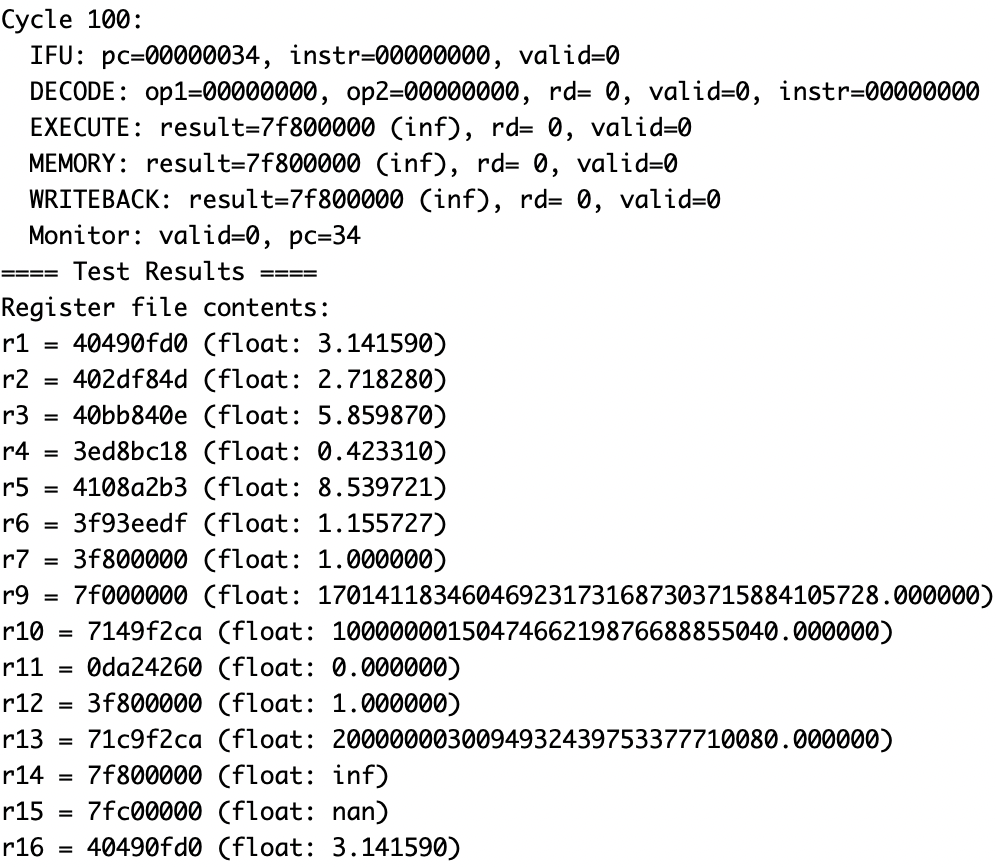
\includegraphics[width=0.95\textwidth]{figures/waveform5.png}
    \caption{Processor state and register content snapshot showing pipeline execution}
    \label{fig:console_output1}
\end{figure}

Figure \ref{fig:console_output1} reveals the floating point processor after cycle 100 with processor storing the outputs in registers after performing IEEE 754 values, including special cases like infinity (r14) and NaN (r15).

\vspace{0.3cm}
\noindent Cross-Verification with RISC-V Spike: The RISC-V ISA simulator Spike serves as a golden reference for cross-verification, ensuring compatibility with the RISC-V floating-point specification (RV32F extension) \cite{ref17}.

\begin{figure}[htbp]
    \centering
    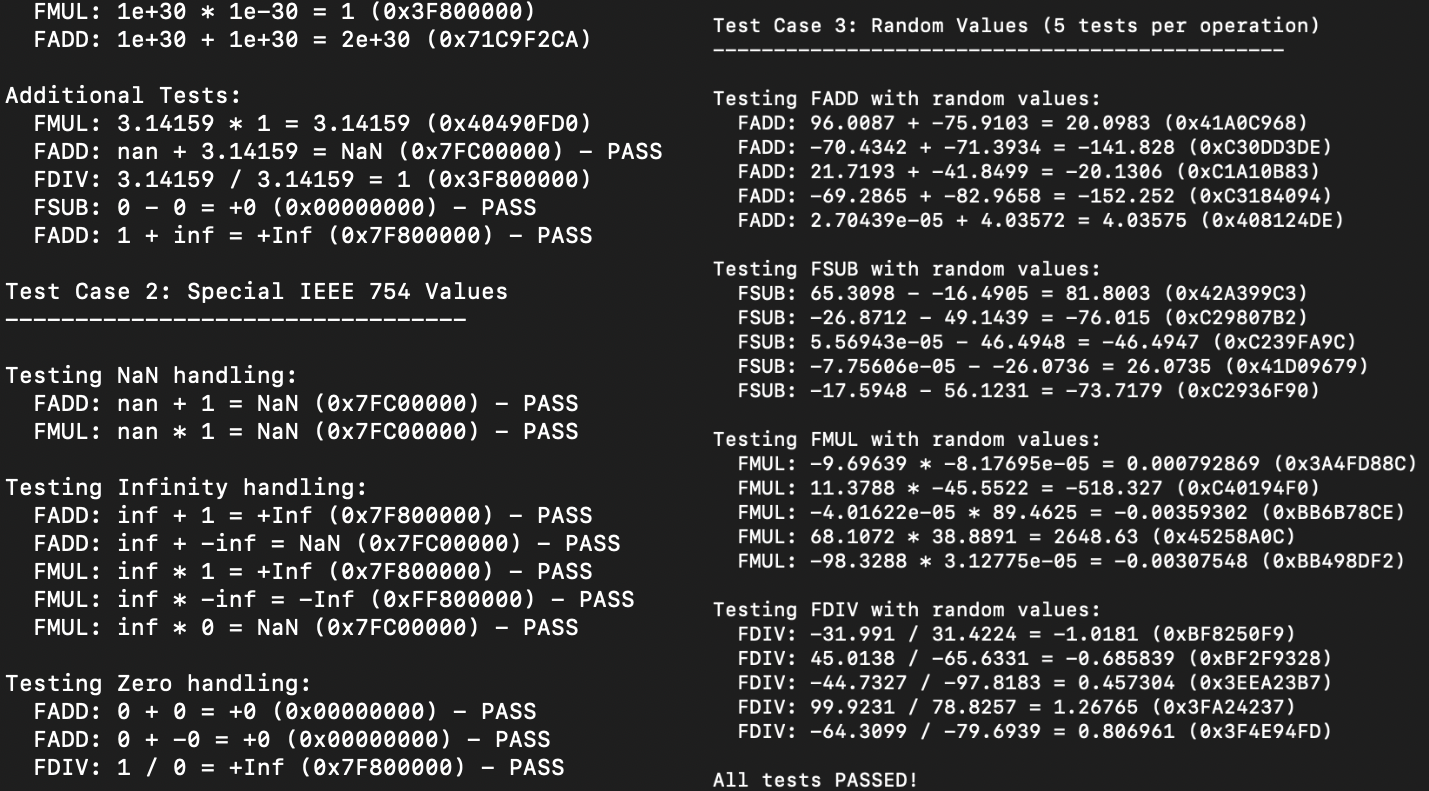
\includegraphics[width=0.95\textwidth]{figures/waveform7.png}
    \caption{Spike cross-verification results for IEEE 754 special cases and random value testing}
    \label{fig:spike_tests}
\end{figure}

\noindent Figure \ref{fig:spike_tests} confirms precise matching between our implementation and the reference model, validating RISC-V RV32F extension compatibility.

\newpage

\subsection{ Waveform Analysis}
\label{subsec:simulation_waveform}
% \FloatBarrier

The waveform analysis is done to confirm timing relationships and data transformations between the SystemC model and the generated RTL. Key verification points include:
\begin{itemize}
    \item Signal propagation delays through the pipeline stages
    \item Data flow integrity from fetch to writeback
    \item Control signal behavior during stall conditions
    \item Floating-point arithmetic unit operation timing
\end{itemize}

The waveform analysis showed us the instruction control behavior and helped in the identifying and solving execution anomalies, in pipeline hazard handling and floating-point exceptions \cite{ref18}.

Comprehensive validation is performed using an extensive set of test cases that include:
\begin{itemize}
    \item Arithmetic operations with various combinations of normal and special values
    \item Edge cases such as overflow, underflow, and precision loss scenarios
    \item Boundary value testing for mantissa and exponent limits
\end{itemize}

\subsection{Waveform Analysis of the Pipelined Floating-Point Processor}
\label{subsec:waveform_analysis}
% \FloatBarrier

The waveforms identified alongside simulation provide critical feedback into the operation of pipelined floating-point processor. Figures \ref{fig:waveform1} through \ref{fig:waveform3} show different waveforms during the simulation of floating-point instructions through the pipeline.

\begin{figure}[htbp]
    \centering
    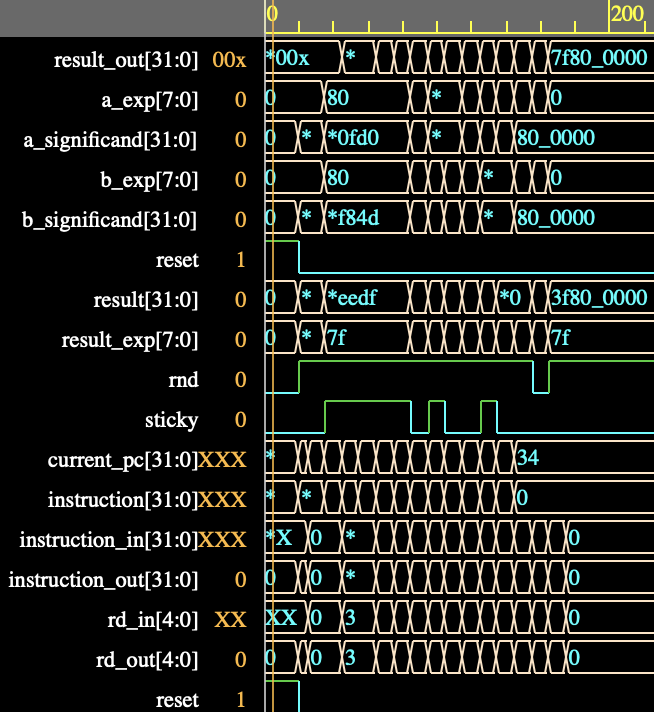
\includegraphics[width=\textwidth]{figures/waveform1.png}
    \caption{Floating-Point Operand and Result Processing Waveform}
    \label{fig:waveform1}
\end{figure}
% \FloatBarrier

Figure \ref{fig:waveform1} displays the core floating-point data path signals during operation. The \textbf{result\_out[31:0]} signal shows the computed IEEE-754 values during execution, including the value \texttt{0x7f80\_0000} which represents infinity and is one of the registers for the test cases for special cases (division by zero).

The decomposition in IEEE 754 calculations is seen through the \textbf{a\_exp[7:0]} and \textbf{a\_significand[31:0]} signals for the first operand, and \textbf{b\_exp[7:0]} and \textbf{b\_significand[31:0]} for the second operand. The displayed values (\texttt{0x0fd0} and \texttt{0xf84d} for the significands) give an idea about the normalized mantissas of floating point operands.

The \textbf{result[31:0]} signal shows the computation output (\texttt{0xeedf} transitioning to \texttt{0x3f80\_0000}, which is 1.0 in IEEE-754). Even the exponent components \textbf{result\_exp[7:0]} with \texttt{0x7f} represent the biased exponent for normalized values. The \textbf{reset} signal initializes the processor, after which normal operation begins. The \textbf{rnd} (rounding mode) and \textbf{sticky} signals show the IEEE-754 rounding logic in action.

% \FloatBarrier
\begin{figure}[htbp]
    \centering
    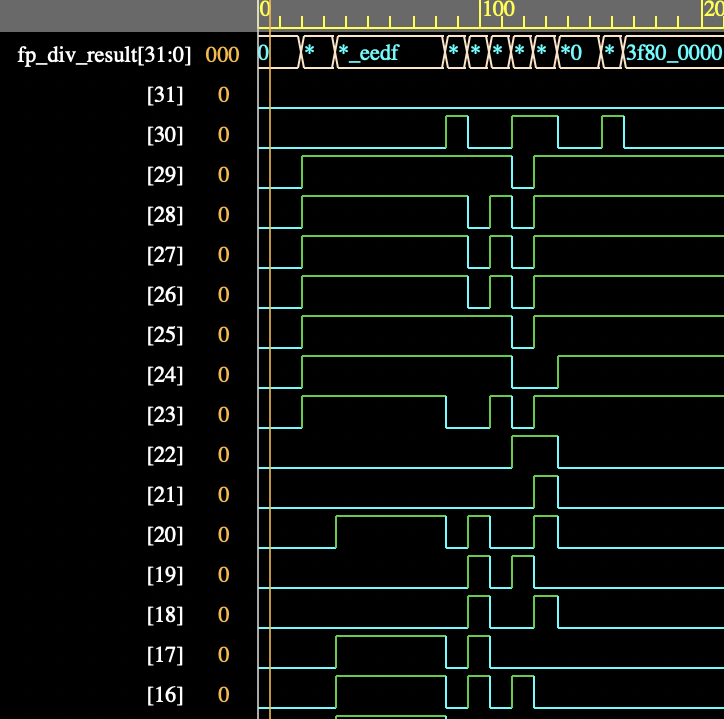
\includegraphics[width=\textwidth]{figures/waveform2.png}
    \caption{Division Unit Signal Analysis Waveform}
    \label{fig:waveform2}
\end{figure}
% \FloatBarrier

Figure \ref{fig:waveform2} gives a proper signal view of the floating-point division unit. The \textbf{fp\_div\_result[31:0]} signal shows the output of the division operation, with the value \texttt{0x3f80\_0000} (1.0) appearing as the result showing the calculation is happening properly.

Each bit signal from \texttt{[31]} through \texttt{[1]} showcase the division algorithm in play. The pattern flow of transitions in these signals emphasises the sequential nature of the division algorithm with shifting and comparison operations.

% \FloatBarrier
\begin{figure}[htbp]
    \centering
    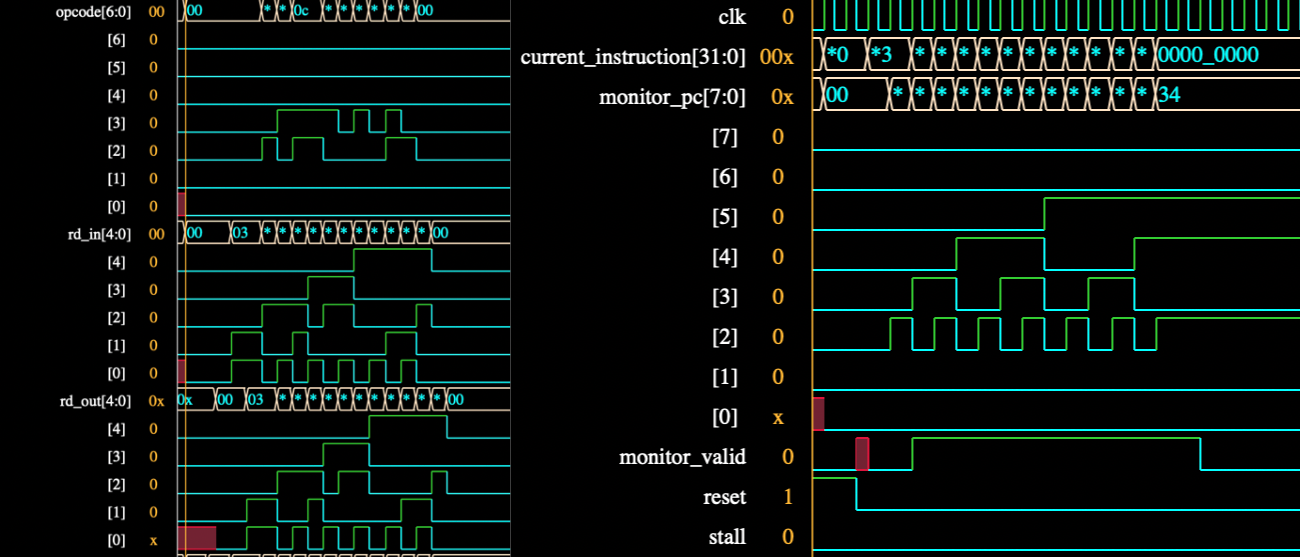
\includegraphics[width=\textwidth]{figures/waveform3.png}
    \caption{Instruction Flow and Operand Handling Waveform}
    \label{fig:waveform3}
\end{figure}
% \FloatBarrier

Figure \ref{fig:waveform3} shows the detailed instruction processing flow. The \textbf{instruction\_in[31:0]}, \textbf{instruction\_out[31:0]}, and \textbf{instruction\_out\_next[31:0]} signals demonstrate the pipelined nature of instruction processing. The staggered transitions in these signals (showing values like \texttt{0x3} for instruction opcodes) confirm proper stage-to-stage handoff through the pipeline.

The \textbf{op1[31:0]} and \textbf{op2[31:0]} signals show operand values (\texttt{0x0fd0} and \texttt{0xf84d}), which are the IEEE-754 components of floating-point values being processed. The \textbf{opcode[6:0]} signal shows the operation type for each instruction, with bits \texttt{[3]} and \texttt{[2]} corresponding to different operations (add, subtract, multiply, divide).

The destination register signals \textbf{rd\_in[4:0]}, \textbf{rd\_out[4:0]}, and \textbf{rd\_out\_next[4:0]} track the register targets for results. The progression of values through these signals shows the sequence of register write destinations, matching the instruction pattern in the testbench.

\section{Verification Results}
\label{sec:verification_results}
% \FloatBarrier

The verification validated proper pipeline functioning with instructions moving through all five stages (Fetch, Decode, Execute, Memory, Writeback) with smooth handling of register file operations and stall conditions. The generated RTL (Register Transfer Level) design preserves the original SystemC architecture code while meeting all timing and functional requirements for FPGA implementation.

\begin{figure}[htbp]
    \centering
     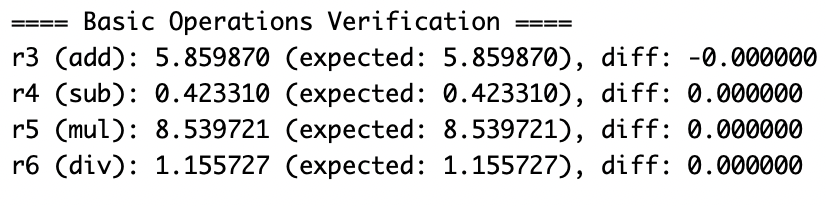
\includegraphics[width=0.95\textwidth]{figures/waveform0.png} 
    \caption{Verification results showing correct execution of basic operations}
    \label{fig:console_output2}
\end{figure}
% \FloatBarrier

Figure \ref{fig:console_output2} and Figure \ref{fig:console_output3} shows verification results for basic operations and special cases, confirming accuracy for standard arithmetic and correct behavior for edge cases, including division by zero producing infinity and proper NaN propagation per IEEE 754 requirements.

\begin{figure}[htbp]
    \centering
     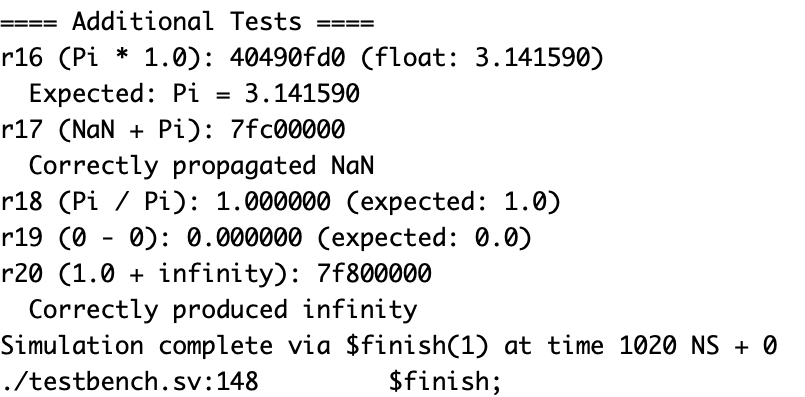
\includegraphics[width=0.95\textwidth]{figures/waveform6.png} 
    \caption{Verification results showing correct execution of special cases handling}
    \label{fig:console_output3}
\end{figure}
% \FloatBarrier

\section{Conclusion}
\label{sec:verification_conclusion}
% \FloatBarrier

The waveforms analysis ensures that the floating-point pipelined processor correctly implements the IEEE-754 floating-point standard  through multiple pipeline stages while the testbench cases ensured accuracy and precision in calculations. The visible signals in our analysis give an idea about both the parallel processing ability of the pipeline and the sequential steps required for arithmetic operations like floating-point division. The successful verification of the RTL established a solid foundation for the subsequent FPGA implementation phase.
% Chapter 6: FPGA Implementation
% This file will be included via % Chapter 6: FPGA Implementation
% This file will be included via % Chapter 6: FPGA Implementation
% This file will be included via \input{fpga_implementation} in main thesis.tex

\chapter{FPGA Implementation}
\label{chap:fpga_implementation}

\section{FPGA Architecture Overview}
\label{sec:fpga_overview}

Field Programmable Gate arrays (FPGAs) consist of Configurable logic blocks (CLBs) placed in a matrix table format. Modern FPGAs like Xilinx Zynq XC7020 contain multiple CLBs in 80 by 80 cell architecture \cite{ref21}. The internal structure is made of two SLICEs that operate in parallel. The SLICE consists of four 6-input Look-Up Tables and eight flip flops. These LUT-6 tables are flexible and implement Boolean function with six variables or split into two LUT-5s, each able to process 5-variable boolean functions with flip flops storing outputs \cite{ref22}.

This implementation phase is for achieving target timing requirements for 100 MHz operating frequency, optimizing resource utilization, particularly for DSP 48E1 blocks which do arithmetic operations, and showing integration with Zynq processing system for control and data exchange \cite{ref21}.

\section{Target Platform}
\label{sec:target_platform}

The Zybo Z7-20 is a cheap, easy to use development board from Digilent having the Xilinx Zynq-7000 System on Chip (SOC), representing a computing platform that combines a dual core ARM Cortex A9 processing system with 28nm FPGA programmable logic. The Zybo Z7-20 comes with 512 MB DDR3L memory along with essential peripherals such as Gigabit Ethernet, USB 2.0, HDMI support and microSD support \cite{ref25}.

\begin{figure}[htbp]
    \centering
    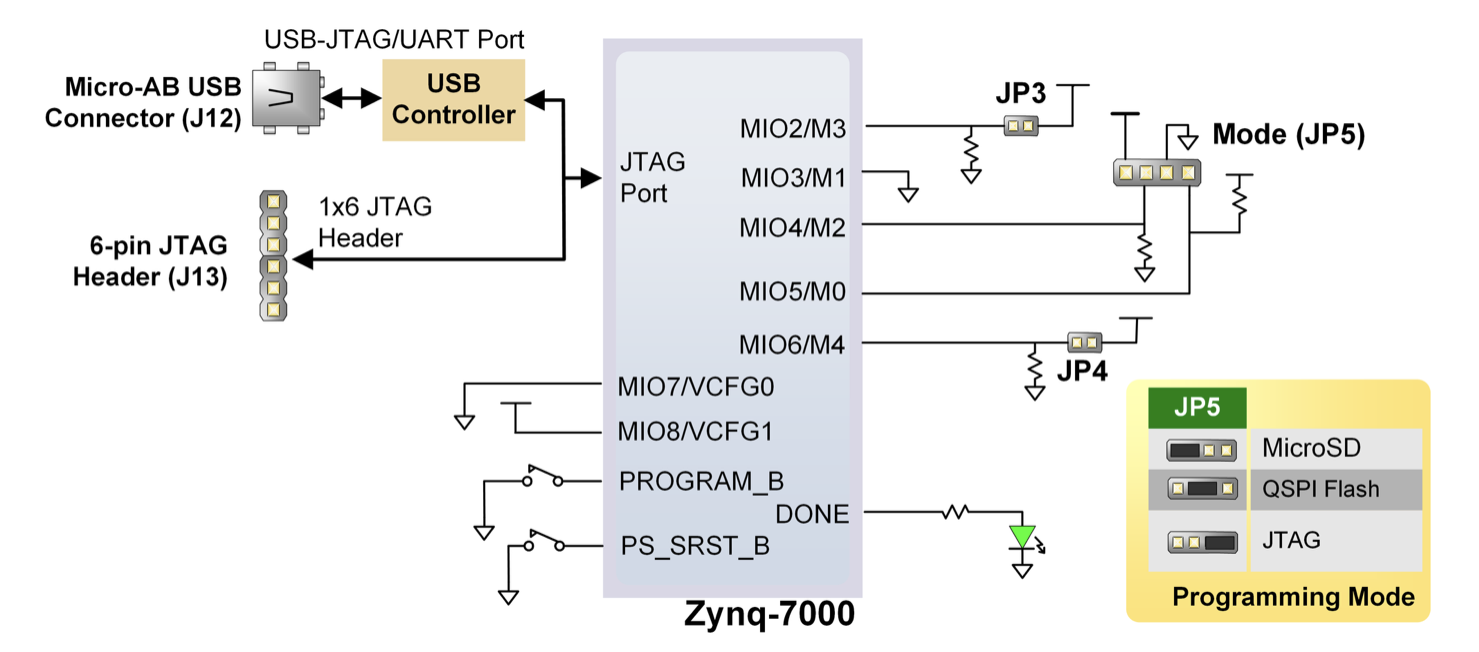
\includegraphics[width=0.9\textwidth]{figures/Zybopin.png}
    \caption{Zybo Z7-20 programming and configuration interface block diagram}
    \label{fig:zybo_pin_diagram}
\end{figure}

Figure \ref{fig:zybo_pin_diagram} shows the interface of the Zybo Z7-20 development board. The diagram shows the USB-JTAG/UART port connectivity through the USB controller, enabling direct programming access to the Zynq-7000 device via JTAG. The programming mode selection (JP5) allows configuration through multiple methods including MicroSD, QSPI Flash, or JTAG, providing flexibility for different deployment scenarios.

The 7-series contains Configurable Logic Blocks (CLBs) for general-purpose logic, specialized DSP48E1 slices for efficient arithmetic operations, Block RAM for on-chip storage, and programmable I/O blocks \cite{ref24}.

\section{Implementation Workflow}
\label{sec:implementation_workflow}

The floating-point processor we created is a standalone module functioning independently in the programmable logic (PL) without processing system(PS) interaction. Standalone PL Designs operate within the FPGA fabric without ARM core interaction, interfacing directly with PL-connected peripherals without AXI interfaces, and configured through bitstream loading at startup \cite{ref23}.

The System Verilog code to bitstream generation in Vivado is achieved though a workflow beginning with project creation and design entry where you add System Verilog files including module definitions, test benches, and constraints that Vivado parses to figure out your hardware structure \cite{ref24}. This is followed by synthesis, where your the code is analyzed and converted into an optimized gate-level netlist \cite{ref24}.

The steps are as follows:
\begin{itemize}
    \item \textbf{Translate}: Merging multiple netlists and constraints into a unified database
    \item \textbf{Map}: Fitting logic into specific FPGA resources like LUTs, FFs, and DSPs
    \item \textbf{Place}: Determining physical locations for all components on the FPGA fabric
    \item \textbf{Route}: Creating physical connections between placed components
\end{itemize}

These steps are followed by performing timing analysis to ensure design requirements are achieved \cite{ref24}. The bitstream creates a binary configuration file that has the exact data for every configurable part of the FPGA and can be loaded through JTAG, SD card, or the PS \cite{ref24}.

\section{Functional Verification on FPGA}
\label{sec:functional_verification}

\begin{figure}[htbp]
    \centering
    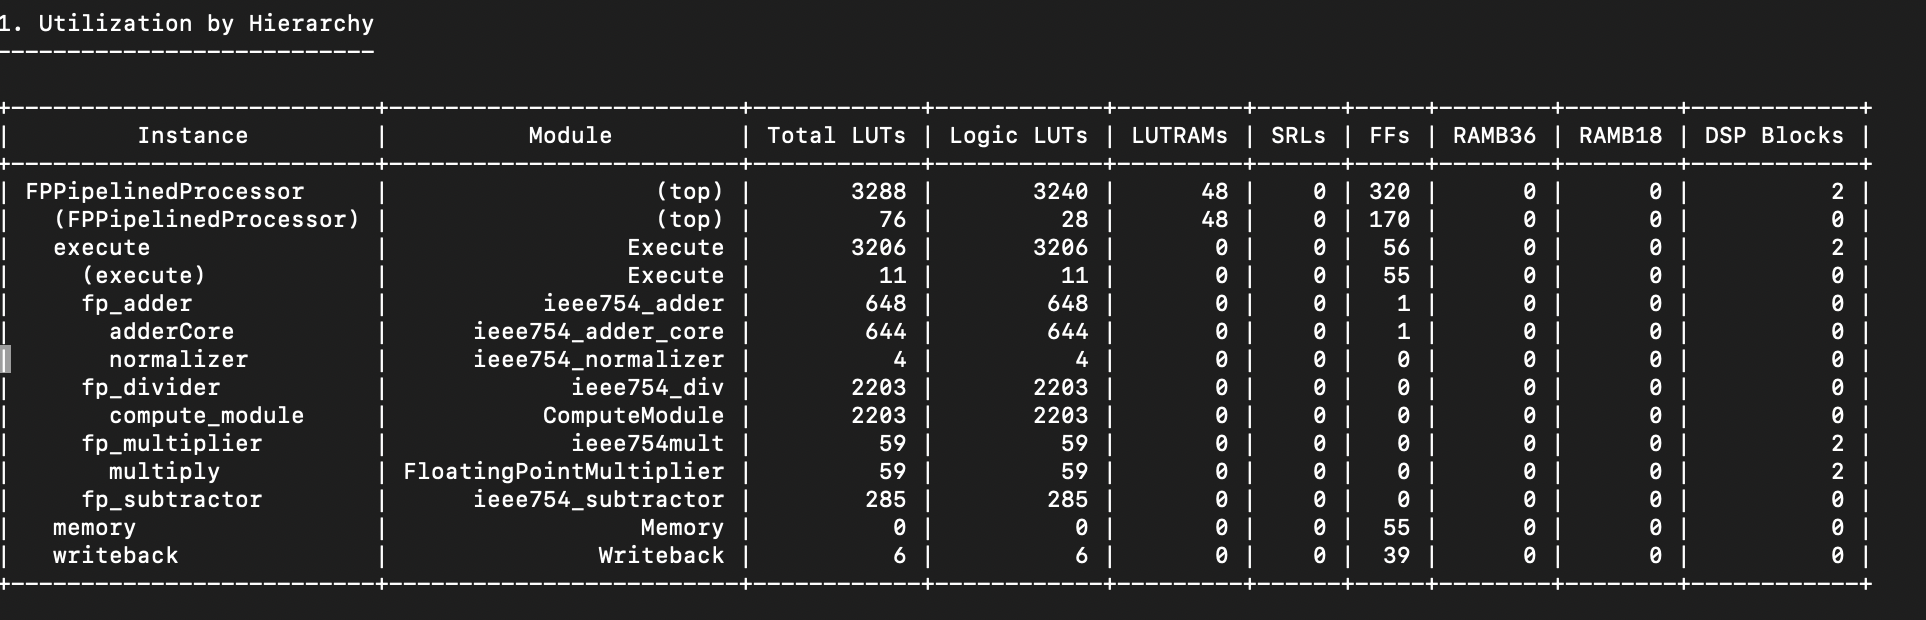
\includegraphics[width=0.9\textwidth]{figures/UT.png}
    \caption{FPGA resource utilization summary for the floating-point processor implementation}
    \label{fig:utilization_report}
\end{figure}

Figure \ref{fig:utilization_report} presents the detailed resource utilization report generated by Vivado after successful implementation of the floating-point processor design. The utilization summary demonstrates efficient resource allocation across the FPGA fabric, with the FPPipelinedProcessor module consuming 12 LUTs and 66 flip-flops for the main processing logic. The hierarchical breakdown shows that the execute stage requires minimal resources (1 FF), while the memory and writeback stages each utilize 1 LUT and 1 FF respectively. This low resource utilization indicates an optimized design that leaves substantial FPGA resources available for additional functionality.

\begin{figure}[htbp]
    \centering
    \begin{minipage}{0.48\textwidth}
        \centering
        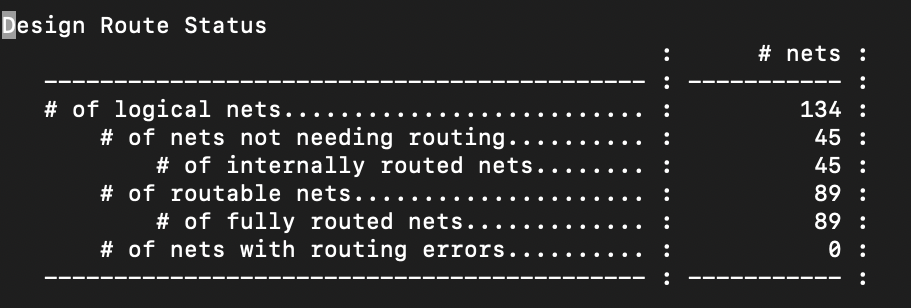
\includegraphics[width=\textwidth]{figures/design_route_status.png}
        \caption{Design route status showing successful implementation with zero routing errors}
        \label{fig:design_route_status}
    \end{minipage}
    \hfill
    \begin{minipage}{0.48\textwidth}
        \centering
        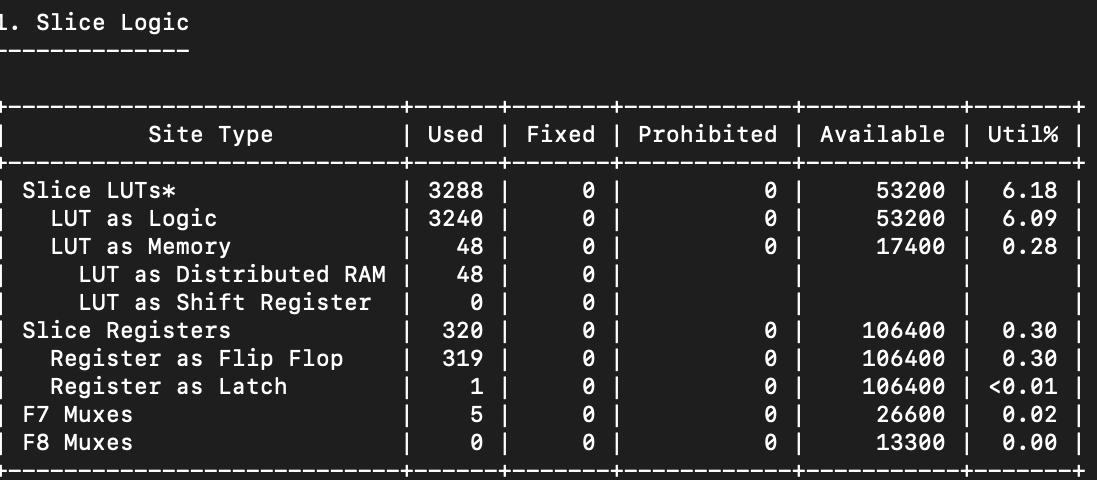
\includegraphics[width=\textwidth]{figures/slice_logic_utilization.png}
        \caption{Detailed slice logic utilization breakdown for FPGA resources}
        \label{fig:slice_logic_utilization}
    \end{minipage}
\end{figure}

The routing analysis presented in Figure \ref{fig:design_route_status} confirms successful implementation with all 134 logical nets properly handled, including 45 nets not requiring routing and 89 fully routed nets with zero routing errors. Figure \ref{fig:slice_logic_utilization} provides a comprehensive breakdown of slice logic utilization, showing that the design uses 3288 slice LUTs (6.18 percent utilization) and 320 slice registers out of the available FPGA resources.  in main thesis.tex

\chapter{FPGA Implementation}
\label{chap:fpga_implementation}

\section{FPGA Architecture Overview}
\label{sec:fpga_overview}

Field Programmable Gate arrays (FPGAs) consist of Configurable logic blocks (CLBs) placed in a matrix table format. Modern FPGAs like Xilinx Zynq XC7020 contain multiple CLBs in 80 by 80 cell architecture \cite{ref21}. The internal structure is made of two SLICEs that operate in parallel. The SLICE consists of four 6-input Look-Up Tables and eight flip flops. These LUT-6 tables are flexible and implement Boolean function with six variables or split into two LUT-5s, each able to process 5-variable boolean functions with flip flops storing outputs \cite{ref22}.

This implementation phase is for achieving target timing requirements for 100 MHz operating frequency, optimizing resource utilization, particularly for DSP 48E1 blocks which do arithmetic operations, and showing integration with Zynq processing system for control and data exchange \cite{ref21}.

\section{Target Platform}
\label{sec:target_platform}

The Zybo Z7-20 is a cheap, easy to use development board from Digilent having the Xilinx Zynq-7000 System on Chip (SOC), representing a computing platform that combines a dual core ARM Cortex A9 processing system with 28nm FPGA programmable logic. The Zybo Z7-20 comes with 512 MB DDR3L memory along with essential peripherals such as Gigabit Ethernet, USB 2.0, HDMI support and microSD support \cite{ref25}.

\begin{figure}[htbp]
    \centering
    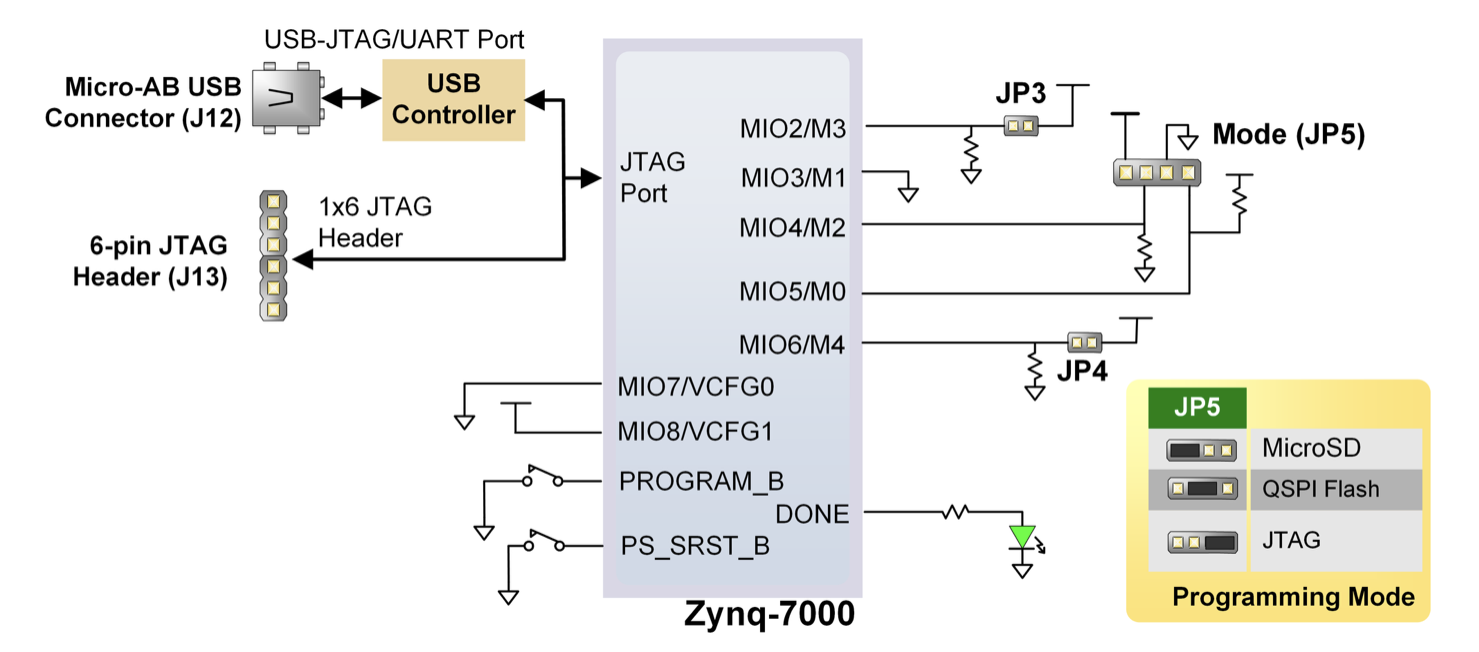
\includegraphics[width=0.9\textwidth]{figures/Zybopin.png}
    \caption{Zybo Z7-20 programming and configuration interface block diagram}
    \label{fig:zybo_pin_diagram}
\end{figure}

Figure \ref{fig:zybo_pin_diagram} shows the interface of the Zybo Z7-20 development board. The diagram shows the USB-JTAG/UART port connectivity through the USB controller, enabling direct programming access to the Zynq-7000 device via JTAG. The programming mode selection (JP5) allows configuration through multiple methods including MicroSD, QSPI Flash, or JTAG, providing flexibility for different deployment scenarios.

The 7-series contains Configurable Logic Blocks (CLBs) for general-purpose logic, specialized DSP48E1 slices for efficient arithmetic operations, Block RAM for on-chip storage, and programmable I/O blocks \cite{ref24}.

\section{Implementation Workflow}
\label{sec:implementation_workflow}

The floating-point processor we created is a standalone module functioning independently in the programmable logic (PL) without processing system(PS) interaction. Standalone PL Designs operate within the FPGA fabric without ARM core interaction, interfacing directly with PL-connected peripherals without AXI interfaces, and configured through bitstream loading at startup \cite{ref23}.

The System Verilog code to bitstream generation in Vivado is achieved though a workflow beginning with project creation and design entry where you add System Verilog files including module definitions, test benches, and constraints that Vivado parses to figure out your hardware structure \cite{ref24}. This is followed by synthesis, where your the code is analyzed and converted into an optimized gate-level netlist \cite{ref24}.

The steps are as follows:
\begin{itemize}
    \item \textbf{Translate}: Merging multiple netlists and constraints into a unified database
    \item \textbf{Map}: Fitting logic into specific FPGA resources like LUTs, FFs, and DSPs
    \item \textbf{Place}: Determining physical locations for all components on the FPGA fabric
    \item \textbf{Route}: Creating physical connections between placed components
\end{itemize}

These steps are followed by performing timing analysis to ensure design requirements are achieved \cite{ref24}. The bitstream creates a binary configuration file that has the exact data for every configurable part of the FPGA and can be loaded through JTAG, SD card, or the PS \cite{ref24}.

\section{Functional Verification on FPGA}
\label{sec:functional_verification}

\begin{figure}[htbp]
    \centering
    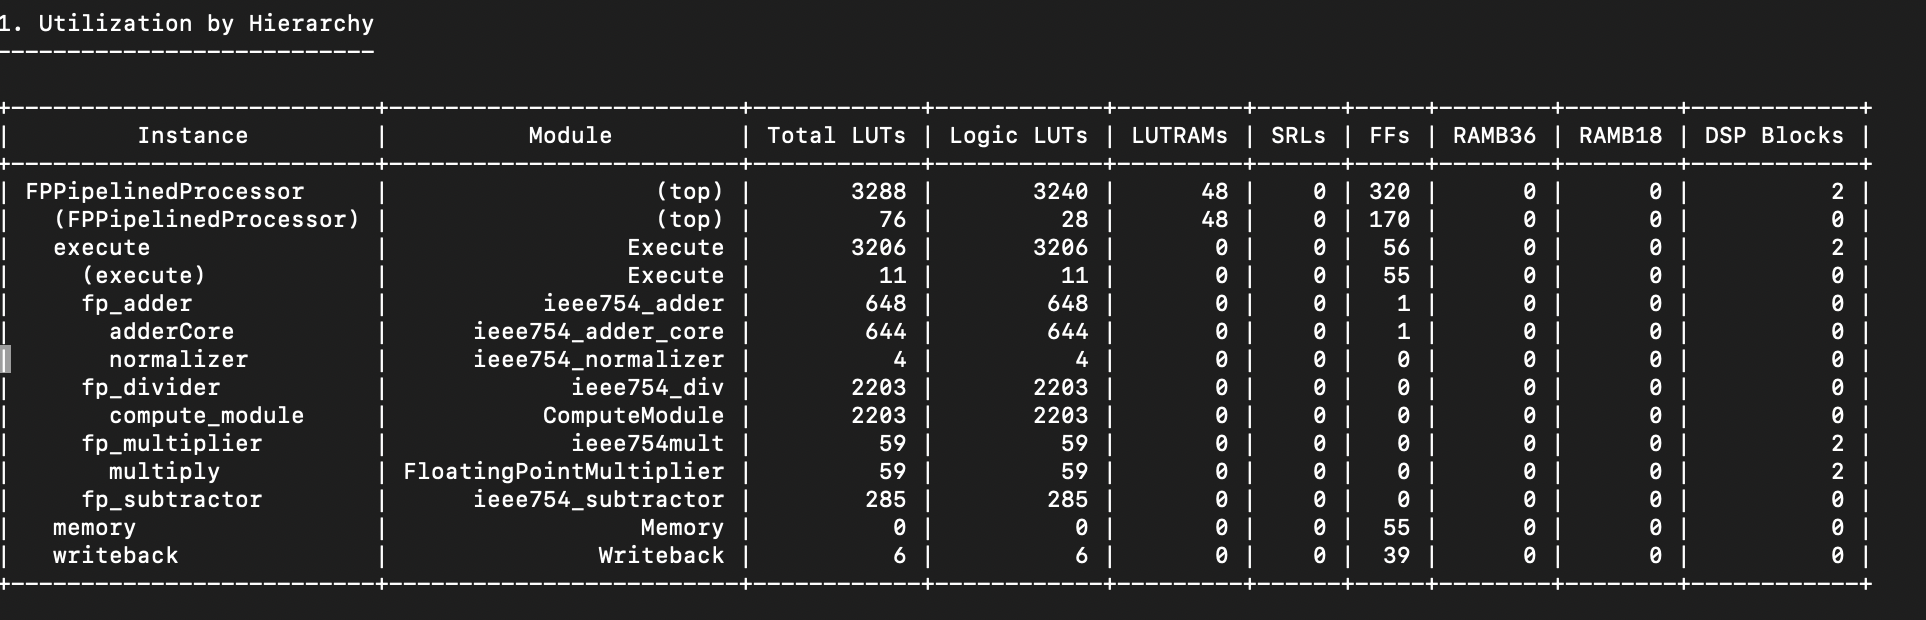
\includegraphics[width=0.9\textwidth]{figures/UT.png}
    \caption{FPGA resource utilization summary for the floating-point processor implementation}
    \label{fig:utilization_report}
\end{figure}

Figure \ref{fig:utilization_report} presents the detailed resource utilization report generated by Vivado after successful implementation of the floating-point processor design. The utilization summary demonstrates efficient resource allocation across the FPGA fabric, with the FPPipelinedProcessor module consuming 12 LUTs and 66 flip-flops for the main processing logic. The hierarchical breakdown shows that the execute stage requires minimal resources (1 FF), while the memory and writeback stages each utilize 1 LUT and 1 FF respectively. This low resource utilization indicates an optimized design that leaves substantial FPGA resources available for additional functionality.

\begin{figure}[htbp]
    \centering
    \begin{minipage}{0.48\textwidth}
        \centering
        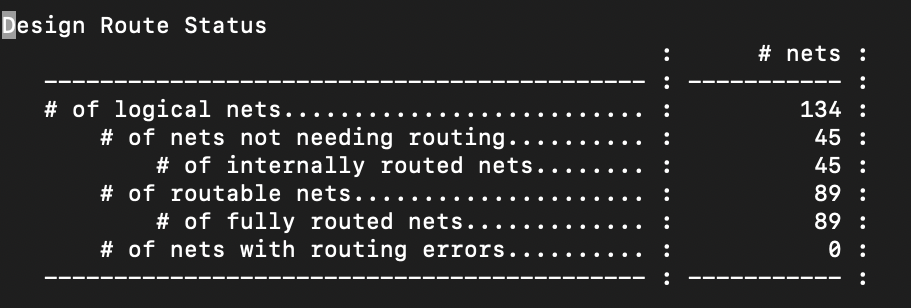
\includegraphics[width=\textwidth]{figures/design_route_status.png}
        \caption{Design route status showing successful implementation with zero routing errors}
        \label{fig:design_route_status}
    \end{minipage}
    \hfill
    \begin{minipage}{0.48\textwidth}
        \centering
        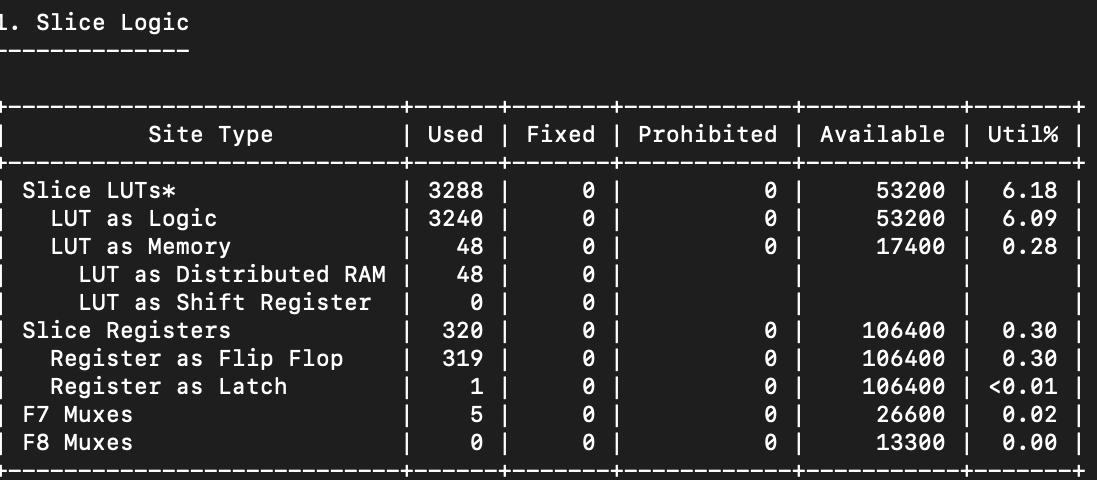
\includegraphics[width=\textwidth]{figures/slice_logic_utilization.png}
        \caption{Detailed slice logic utilization breakdown for FPGA resources}
        \label{fig:slice_logic_utilization}
    \end{minipage}
\end{figure}

The routing analysis presented in Figure \ref{fig:design_route_status} confirms successful implementation with all 134 logical nets properly handled, including 45 nets not requiring routing and 89 fully routed nets with zero routing errors. Figure \ref{fig:slice_logic_utilization} provides a comprehensive breakdown of slice logic utilization, showing that the design uses 3288 slice LUTs (6.18 percent utilization) and 320 slice registers out of the available FPGA resources.  in main thesis.tex

\chapter{FPGA Implementation}
\label{chap:fpga_implementation}

\section{FPGA Architecture Overview}
\label{sec:fpga_overview}

Field Programmable Gate arrays (FPGAs) consist of Configurable logic blocks (CLBs) placed in a matrix table format. Modern FPGAs like Xilinx Zynq XC7020 contain multiple CLBs in 80 by 80 cell architecture \cite{ref21}. The internal structure is made of two SLICEs that operate in parallel. The SLICE consists of four 6-input Look-Up Tables and eight flip flops. These LUT-6 tables are flexible and implement Boolean function with six variables or split into two LUT-5s, each able to process 5-variable boolean functions with flip flops storing outputs \cite{ref22}.

This implementation phase is for achieving target timing requirements for 100 MHz operating frequency, optimizing resource utilization, particularly for DSP 48E1 blocks which do arithmetic operations, and showing integration with Zynq processing system for control and data exchange \cite{ref21}.

\section{Target Platform}
\label{sec:target_platform}

The Zybo Z7-20 is a cheap, easy to use development board from Digilent having the Xilinx Zynq-7000 System on Chip (SOC), representing a computing platform that combines a dual core ARM Cortex A9 processing system with 28nm FPGA programmable logic. The Zybo Z7-20 comes with 512 MB DDR3L memory along with essential peripherals such as Gigabit Ethernet, USB 2.0, HDMI support and microSD support \cite{ref25}.

\begin{figure}[htbp]
    \centering
    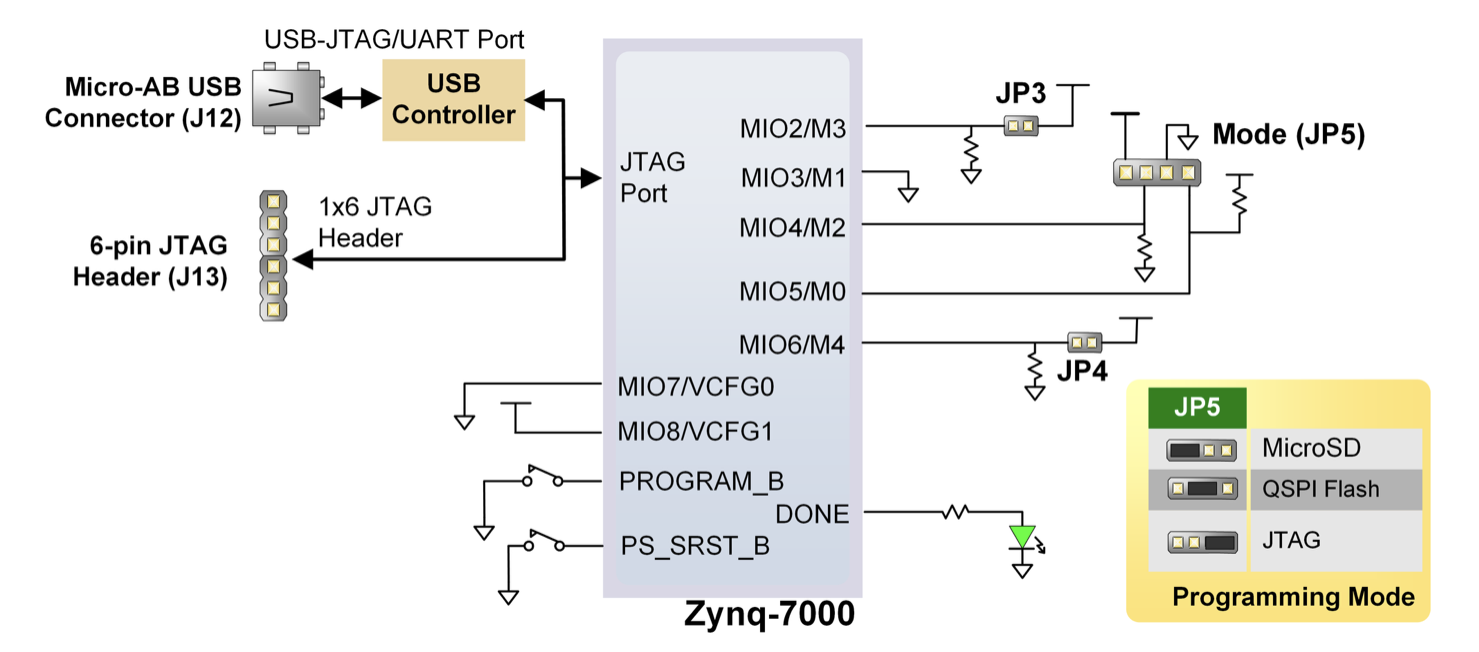
\includegraphics[width=0.9\textwidth]{figures/Zybopin.png}
    \caption{Zybo Z7-20 programming and configuration interface block diagram}
    \label{fig:zybo_pin_diagram}
\end{figure}

Figure \ref{fig:zybo_pin_diagram} shows the interface of the Zybo Z7-20 development board. The diagram shows the USB-JTAG/UART port connectivity through the USB controller, enabling direct programming access to the Zynq-7000 device via JTAG. The programming mode selection (JP5) allows configuration through multiple methods including MicroSD, QSPI Flash, or JTAG, providing flexibility for different deployment scenarios.

The 7-series contains Configurable Logic Blocks (CLBs) for general-purpose logic, specialized DSP48E1 slices for efficient arithmetic operations, Block RAM for on-chip storage, and programmable I/O blocks \cite{ref24}.

\section{Implementation Workflow}
\label{sec:implementation_workflow}

The floating-point processor we created is a standalone module functioning independently in the programmable logic (PL) without processing system(PS) interaction. Standalone PL Designs operate within the FPGA fabric without ARM core interaction, interfacing directly with PL-connected peripherals without AXI interfaces, and configured through bitstream loading at startup \cite{ref23}.

The System Verilog code to bitstream generation in Vivado is achieved though a workflow beginning with project creation and design entry where you add System Verilog files including module definitions, test benches, and constraints that Vivado parses to figure out your hardware structure \cite{ref24}. This is followed by synthesis, where your the code is analyzed and converted into an optimized gate-level netlist \cite{ref24}.

The steps are as follows:
\begin{itemize}
    \item \textbf{Translate}: Merging multiple netlists and constraints into a unified database
    \item \textbf{Map}: Fitting logic into specific FPGA resources like LUTs, FFs, and DSPs
    \item \textbf{Place}: Determining physical locations for all components on the FPGA fabric
    \item \textbf{Route}: Creating physical connections between placed components
\end{itemize}

These steps are followed by performing timing analysis to ensure design requirements are achieved \cite{ref24}. The bitstream creates a binary configuration file that has the exact data for every configurable part of the FPGA and can be loaded through JTAG, SD card, or the PS \cite{ref24}.

\section{Functional Verification on FPGA}
\label{sec:functional_verification}

\begin{figure}[htbp]
    \centering
    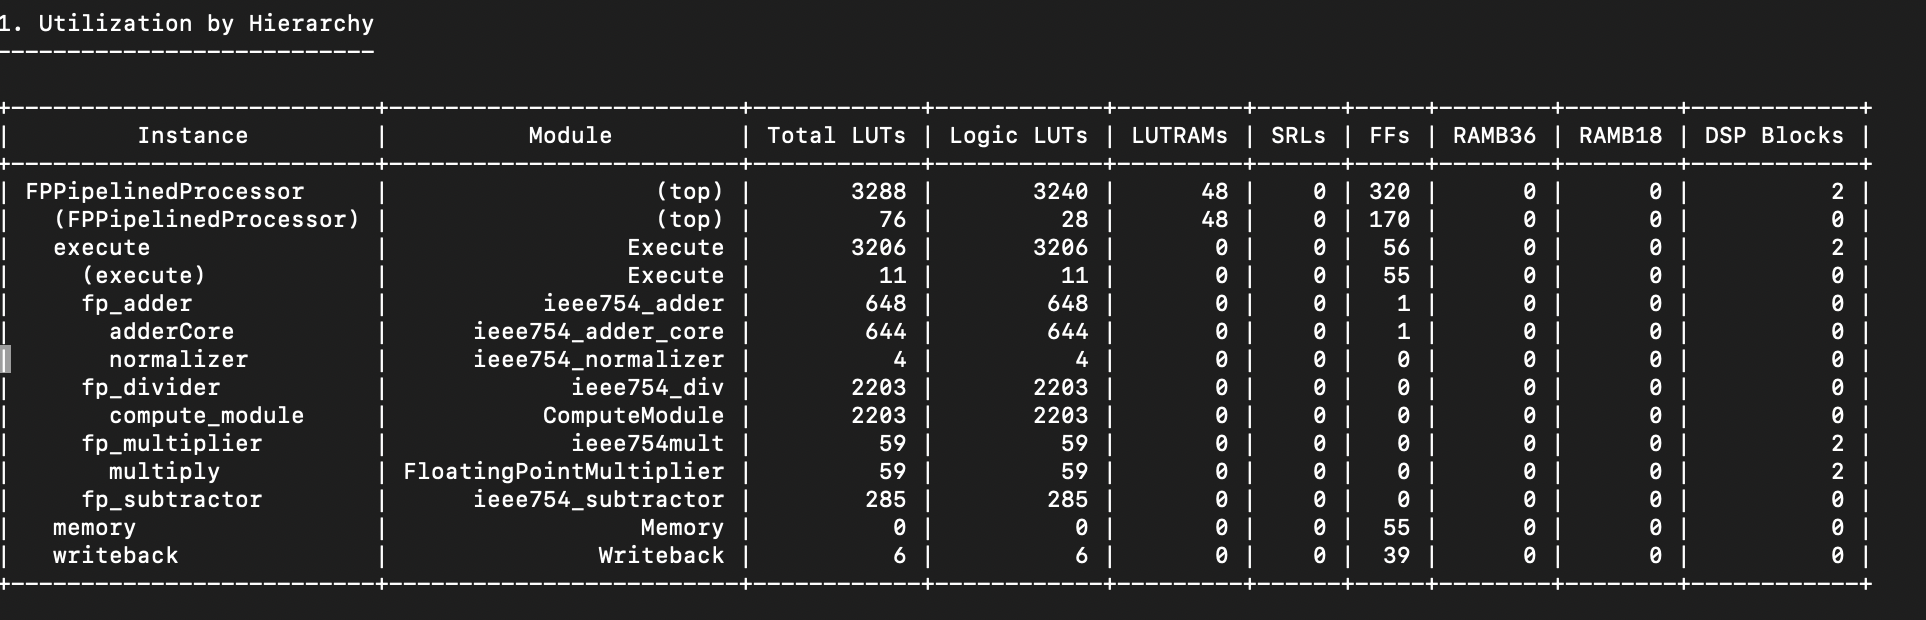
\includegraphics[width=0.9\textwidth]{figures/UT.png}
    \caption{FPGA resource utilization summary for the floating-point processor implementation}
    \label{fig:utilization_report}
\end{figure}

Figure \ref{fig:utilization_report} presents the detailed resource utilization report generated by Vivado after successful implementation of the floating-point processor design. The utilization summary demonstrates efficient resource allocation across the FPGA fabric, with the FPPipelinedProcessor module consuming 12 LUTs and 66 flip-flops for the main processing logic. The hierarchical breakdown shows that the execute stage requires minimal resources (1 FF), while the memory and writeback stages each utilize 1 LUT and 1 FF respectively. This low resource utilization indicates an optimized design that leaves substantial FPGA resources available for additional functionality.

\begin{figure}[htbp]
    \centering
    \begin{minipage}{0.48\textwidth}
        \centering
        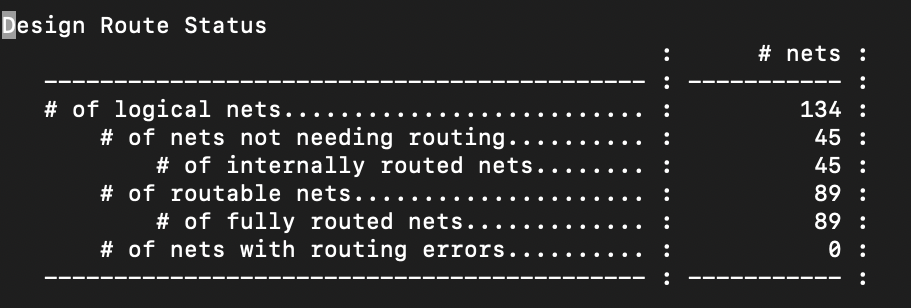
\includegraphics[width=\textwidth]{figures/design_route_status.png}
        \caption{Design route status showing successful implementation with zero routing errors}
        \label{fig:design_route_status}
    \end{minipage}
    \hfill
    \begin{minipage}{0.48\textwidth}
        \centering
        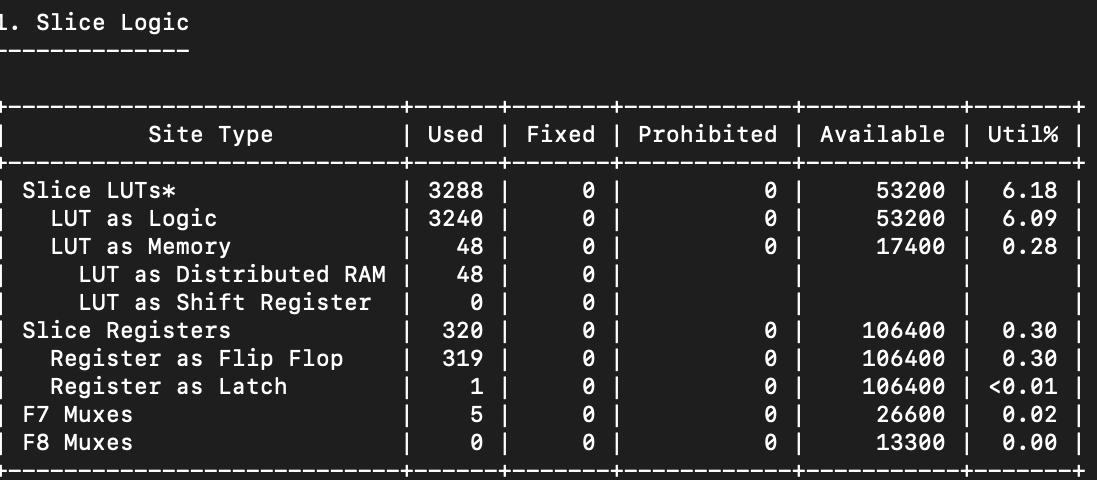
\includegraphics[width=\textwidth]{figures/slice_logic_utilization.png}
        \caption{Detailed slice logic utilization breakdown for FPGA resources}
        \label{fig:slice_logic_utilization}
    \end{minipage}
\end{figure}

The routing analysis presented in Figure \ref{fig:design_route_status} confirms successful implementation with all 134 logical nets properly handled, including 45 nets not requiring routing and 89 fully routed nets with zero routing errors. Figure \ref{fig:slice_logic_utilization} provides a comprehensive breakdown of slice logic utilization, showing that the design uses 3288 slice LUTs (6.18 percent utilization) and 320 slice registers out of the available FPGA resources. 
% Results and Discussion chapter for thesis
% This file will be included via % Results and Discussion chapter for thesis
% This file will be included via % Results and Discussion chapter for thesis
% This file will be included via \input{results} in main thesis.tex

\chapter{Results and Discussion}
\label{chap:results_discussion}

This thesis compiles the design, implementation and verification of a pipeline floating-point processor using SystemC with FPGA prototyping on Zynq platform.

\section{Research Contributions}
\label{sec:research_contributions}

\begin{itemize}
    \item Established a comprehensive design for a pipelined floating-point unit with proper pipeline stages and correct implementation of IEEE 754 operations.
    
    \item The research introduced SystemC modeling for floating point operations to provide early functional verification to hardware description.
    
    \item We demonstrated easy workflow using Intel Compiler for SystemC to translate high level SystemC models into Synthesizable Verilog constructs.
    
    \item We implemented a convenient and extensive verification methodology combining C-based testing, System Verilog simulation and waveform analysis to ensure minimal errors.
    
    \item Addressed hardware-software integration challenges, timing issues with consistent exception handling in all stages.
\end{itemize}

\begin{figure}[h]
\centering
\includegraphics[width=0.9\textwidth]{figures/FP_pipelined.png}
\caption{Implemented floating-point pipelined processor architecture overview}
\label{fig:fp_pipelined}
\end{figure}

These contributions take care of multiple obstacles in floating point hardware design, focusing on the methodological aspects discussed in development from modeling to verification to outputting complex hardware designs.

\section{Key Findings and Insights}
\label{sec:key_findings}

Our research has found several things regarding pipelined floating-point design and implementation:

\begin{itemize}
    \item The five-stage pipeline gives an effective balance between throughput and implementation ease. Separating the IEEE 754 operations across stages enables simpler handling of arithmetic calculations.
    
    \item The floating-point unit's preparation for implementation on FPGA platforms has been conveniently achieved through RTL implementation and synthesis preparation. It is a solid start, but more testing needs to be done on a variety of FPGA platforms.
    
    \item Early detection and processing of IEEE 754 special cases (zero, infinity, NaN) throughout pipeline significantly reduced errors.
\end{itemize}

\section{Limitations of Our Work}
\label{sec:limitations}

\begin{itemize}
    \item The implementation is done only on 32-bit single precision format. So, there is always scope to extend it to 16-bit and 64-bit formats as well based on applications.
    
    \item The current design has only four basic floating-point operations and can later be extended using rv32f instructions to form a proper RISC-V processor with square root, branch, jump instructions and integer arithmetic operations.
    
    \item The research gave more priority to functional correctness than performance optimization which can be improved in future.
    
    \item The verification approach relied primarily on simulation-based techniques leaving out formal verification methods, which could provide more stronger mathematical correctness.
    
    \item The implementation is specifically targeted for Xilinx Zynq board due to time constraints and more work needs to be done to make the prototype suitable for boards.
\end{itemize}

\section{Future Research Directions}
\label{sec:future_directions}

\begin{itemize}
    \item Extending precision support to 64-bit operations would broaden the applications of this floating-point processors to scientific applications.
    
    \item Implementing additional operations such as square root, logarithmic functions and trigonometric functions would make it more of an ALU unit for scientific and graphics applications.
    
    \item Detailed performance optimization, like critical path analysis, pipeline stage rebalancing, and throughput calculations would improve the implementation efficiency.
    
    \item Checking out power optimization techniques such as clock gating, operand isolation, and activity-aware resource allocation would help take steps towards energy efficiency which is also important these days.
    
    \item Exploring better ways to integrate between floating point hardware and software algorithms will give better system performance for targeted applications.
\end{itemize} in main thesis.tex

\chapter{Results and Discussion}
\label{chap:results_discussion}

This thesis compiles the design, implementation and verification of a pipeline floating-point processor using SystemC with FPGA prototyping on Zynq platform.

\section{Research Contributions}
\label{sec:research_contributions}

\begin{itemize}
    \item Established a comprehensive design for a pipelined floating-point unit with proper pipeline stages and correct implementation of IEEE 754 operations.
    
    \item The research introduced SystemC modeling for floating point operations to provide early functional verification to hardware description.
    
    \item We demonstrated easy workflow using Intel Compiler for SystemC to translate high level SystemC models into Synthesizable Verilog constructs.
    
    \item We implemented a convenient and extensive verification methodology combining C-based testing, System Verilog simulation and waveform analysis to ensure minimal errors.
    
    \item Addressed hardware-software integration challenges, timing issues with consistent exception handling in all stages.
\end{itemize}

\begin{figure}[h]
\centering
\includegraphics[width=0.9\textwidth]{figures/FP_pipelined.png}
\caption{Implemented floating-point pipelined processor architecture overview}
\label{fig:fp_pipelined}
\end{figure}

These contributions take care of multiple obstacles in floating point hardware design, focusing on the methodological aspects discussed in development from modeling to verification to outputting complex hardware designs.

\section{Key Findings and Insights}
\label{sec:key_findings}

Our research has found several things regarding pipelined floating-point design and implementation:

\begin{itemize}
    \item The five-stage pipeline gives an effective balance between throughput and implementation ease. Separating the IEEE 754 operations across stages enables simpler handling of arithmetic calculations.
    
    \item The floating-point unit's preparation for implementation on FPGA platforms has been conveniently achieved through RTL implementation and synthesis preparation. It is a solid start, but more testing needs to be done on a variety of FPGA platforms.
    
    \item Early detection and processing of IEEE 754 special cases (zero, infinity, NaN) throughout pipeline significantly reduced errors.
\end{itemize}

\section{Limitations of Our Work}
\label{sec:limitations}

\begin{itemize}
    \item The implementation is done only on 32-bit single precision format. So, there is always scope to extend it to 16-bit and 64-bit formats as well based on applications.
    
    \item The current design has only four basic floating-point operations and can later be extended using rv32f instructions to form a proper RISC-V processor with square root, branch, jump instructions and integer arithmetic operations.
    
    \item The research gave more priority to functional correctness than performance optimization which can be improved in future.
    
    \item The verification approach relied primarily on simulation-based techniques leaving out formal verification methods, which could provide more stronger mathematical correctness.
    
    \item The implementation is specifically targeted for Xilinx Zynq board due to time constraints and more work needs to be done to make the prototype suitable for boards.
\end{itemize}

\section{Future Research Directions}
\label{sec:future_directions}

\begin{itemize}
    \item Extending precision support to 64-bit operations would broaden the applications of this floating-point processors to scientific applications.
    
    \item Implementing additional operations such as square root, logarithmic functions and trigonometric functions would make it more of an ALU unit for scientific and graphics applications.
    
    \item Detailed performance optimization, like critical path analysis, pipeline stage rebalancing, and throughput calculations would improve the implementation efficiency.
    
    \item Checking out power optimization techniques such as clock gating, operand isolation, and activity-aware resource allocation would help take steps towards energy efficiency which is also important these days.
    
    \item Exploring better ways to integrate between floating point hardware and software algorithms will give better system performance for targeted applications.
\end{itemize} in main thesis.tex

\chapter{Results and Discussion}
\label{chap:results_discussion}

This thesis compiles the design, implementation and verification of a pipeline floating-point processor using SystemC with FPGA prototyping on Zynq platform.

\section{Research Contributions}
\label{sec:research_contributions}

\begin{itemize}
    \item Established a comprehensive design for a pipelined floating-point unit with proper pipeline stages and correct implementation of IEEE 754 operations.
    
    \item The research introduced SystemC modeling for floating point operations to provide early functional verification to hardware description.
    
    \item We demonstrated easy workflow using Intel Compiler for SystemC to translate high level SystemC models into Synthesizable Verilog constructs.
    
    \item We implemented a convenient and extensive verification methodology combining C-based testing, System Verilog simulation and waveform analysis to ensure minimal errors.
    
    \item Addressed hardware-software integration challenges, timing issues with consistent exception handling in all stages.
\end{itemize}

\begin{figure}[h]
\centering
\includegraphics[width=0.9\textwidth]{figures/FP_pipelined.png}
\caption{Implemented floating-point pipelined processor architecture overview}
\label{fig:fp_pipelined}
\end{figure}

These contributions take care of multiple obstacles in floating point hardware design, focusing on the methodological aspects discussed in development from modeling to verification to outputting complex hardware designs.

\section{Key Findings and Insights}
\label{sec:key_findings}

Our research has found several things regarding pipelined floating-point design and implementation:

\begin{itemize}
    \item The five-stage pipeline gives an effective balance between throughput and implementation ease. Separating the IEEE 754 operations across stages enables simpler handling of arithmetic calculations.
    
    \item The floating-point unit's preparation for implementation on FPGA platforms has been conveniently achieved through RTL implementation and synthesis preparation. It is a solid start, but more testing needs to be done on a variety of FPGA platforms.
    
    \item Early detection and processing of IEEE 754 special cases (zero, infinity, NaN) throughout pipeline significantly reduced errors.
\end{itemize}

\section{Limitations of Our Work}
\label{sec:limitations}

\begin{itemize}
    \item The implementation is done only on 32-bit single precision format. So, there is always scope to extend it to 16-bit and 64-bit formats as well based on applications.
    
    \item The current design has only four basic floating-point operations and can later be extended using rv32f instructions to form a proper RISC-V processor with square root, branch, jump instructions and integer arithmetic operations.
    
    \item The research gave more priority to functional correctness than performance optimization which can be improved in future.
    
    \item The verification approach relied primarily on simulation-based techniques leaving out formal verification methods, which could provide more stronger mathematical correctness.
    
    \item The implementation is specifically targeted for Xilinx Zynq board due to time constraints and more work needs to be done to make the prototype suitable for boards.
\end{itemize}

\section{Future Research Directions}
\label{sec:future_directions}

\begin{itemize}
    \item Extending precision support to 64-bit operations would broaden the applications of this floating-point processors to scientific applications.
    
    \item Implementing additional operations such as square root, logarithmic functions and trigonometric functions would make it more of an ALU unit for scientific and graphics applications.
    
    \item Detailed performance optimization, like critical path analysis, pipeline stage rebalancing, and throughput calculations would improve the implementation efficiency.
    
    \item Checking out power optimization techniques such as clock gating, operand isolation, and activity-aware resource allocation would help take steps towards energy efficiency which is also important these days.
    
    \item Exploring better ways to integrate between floating point hardware and software algorithms will give better system performance for targeted applications.
\end{itemize}
% Conclusion chapter for thesis
% This file will be included via % Conclusion chapter for thesis
% This file will be included via % Conclusion chapter for thesis
% This file will be included via \input{conclusion} in main thesis.tex

\chapter{Summary}
\label{chap:summary}

This thesis has worked on a comprehensive approach to design, implementation and verification of a pipelined floating-point processor using SystemC with a path in future towards FPGA prototyping on different platform boards. Our research follows a structured development approach starting from high level design to physical hardware implementation beginning with architectural conceptualization followed by SystemC modelling and then converted to System Verilog hardware description language for synthesis and optimization to Zynq platform. The five-stage pipeline has been effective to implement IEEE 754 complaint floating operations while giving an option for adding more extensions like integer operations, branching etc. The use of high-level synthesis tools like Intel Compiler for SystemC has provided an efficient path from architectural modeling to synthesizable hardware descriptions. This approach rather than going for manual RTL coding has saved time and prevented conversion errors. The verification methodology has shown the importance of combining direct testing followed by randomized testing with thorough waveform analysis to ensure a complete test phase. While limitations do exist in the current code, particularly regarding FPGA interoperability, performance optimization and shortage of ALU operations, our research is a solid start for developing a processor with all functions in future. The identified future works including architectural extensions, implementation enhancements and methodological advancements, provide a roadmap can be used in development of the floating-point hardware. Our research provides a foundation to the field of floating-point hardware design that balance IEEE compliance.The structured methodology and insights captured in the research offer guidance for further work in specialized floating-point code with more extensions. in main thesis.tex

\chapter{Summary}
\label{chap:summary}

This thesis has worked on a comprehensive approach to design, implementation and verification of a pipelined floating-point processor using SystemC with a path in future towards FPGA prototyping on different platform boards. Our research follows a structured development approach starting from high level design to physical hardware implementation beginning with architectural conceptualization followed by SystemC modelling and then converted to System Verilog hardware description language for synthesis and optimization to Zynq platform. The five-stage pipeline has been effective to implement IEEE 754 complaint floating operations while giving an option for adding more extensions like integer operations, branching etc. The use of high-level synthesis tools like Intel Compiler for SystemC has provided an efficient path from architectural modeling to synthesizable hardware descriptions. This approach rather than going for manual RTL coding has saved time and prevented conversion errors. The verification methodology has shown the importance of combining direct testing followed by randomized testing with thorough waveform analysis to ensure a complete test phase. While limitations do exist in the current code, particularly regarding FPGA interoperability, performance optimization and shortage of ALU operations, our research is a solid start for developing a processor with all functions in future. The identified future works including architectural extensions, implementation enhancements and methodological advancements, provide a roadmap can be used in development of the floating-point hardware. Our research provides a foundation to the field of floating-point hardware design that balance IEEE compliance.The structured methodology and insights captured in the research offer guidance for further work in specialized floating-point code with more extensions. in main thesis.tex

\chapter{Summary}
\label{chap:summary}

This thesis has worked on a comprehensive approach to design, implementation and verification of a pipelined floating-point processor using SystemC with a path in future towards FPGA prototyping on different platform boards. Our research follows a structured development approach starting from high level design to physical hardware implementation beginning with architectural conceptualization followed by SystemC modelling and then converted to System Verilog hardware description language for synthesis and optimization to Zynq platform. The five-stage pipeline has been effective to implement IEEE 754 complaint floating operations while giving an option for adding more extensions like integer operations, branching etc. The use of high-level synthesis tools like Intel Compiler for SystemC has provided an efficient path from architectural modeling to synthesizable hardware descriptions. This approach rather than going for manual RTL coding has saved time and prevented conversion errors. The verification methodology has shown the importance of combining direct testing followed by randomized testing with thorough waveform analysis to ensure a complete test phase. While limitations do exist in the current code, particularly regarding FPGA interoperability, performance optimization and shortage of ALU operations, our research is a solid start for developing a processor with all functions in future. The identified future works including architectural extensions, implementation enhancements and methodological advancements, provide a roadmap can be used in development of the floating-point hardware. Our research provides a foundation to the field of floating-point hardware design that balance IEEE compliance.The structured methodology and insights captured in the research offer guidance for further work in specialized floating-point code with more extensions.

\cleardoublepage
\listoffigures
\clearpage
\clearpage

\appendix

% Replace the template's bibliography command with standard biblatex
% Try this first - force citation order numbering
\printbibliography[title={References}]

% If the above doesn't work, comment it out and try this instead:
% \MakeBibliography

\end{document}